

\chapter{State of the Art}
\label{sec:state}

This section consists of an application-related part, where I present state-of-the-art approaches and theory on crowd management, and a methods-related part that comprises approaches from computer science for the simulative assessment of a crowd guidance system.


In the first part (Section~\ref{sec:crowdmanagement}), I look at crowd management from a traffic engineering perspective to give an overview of the research field and its application in practice. I identify research gaps that I aim to close in my later investigations. Therefore, the first part is strongly connected to the research questions presented in the introduction. 


In the second part (Sections~\ref{sec:modelcrowd}-\ref{sec:uq}), I look at methodological aspects from a computer science perspective. As I base my investigations on simulations, I look at how the key components of a crowd guidance system, which are the crowd and the mobile network, can be modeled and simulated. In Section~\ref{sec:modelcrowd}, approaches for modeling and simulating crowd behavior are presented. I introduce a hierarchical modeling approach where locomotion is modeled at the operational layer and route choice at the tactical layer. In Section~\ref{sec:modelcom}, I provide an overview of mobile communication standards that specify direct communication and discuss how the respective protocol stacks and the radio channel are modeled and simulated.  
Since crowd and network models are separate models, Section~\ref{sec:simulationframeworks} presents techniques for connecting them. This includes update schemes and techniques for data exchange between simulators. 
It is crucial to quantify errors or uncertainties in the simulation output. Therefore, I present a surrogate-based approach with polynomial chaos expansions in Section~\ref{sec:uq}. 



\section{Crowd Management}

This section belongs to the application-related part of the state of the art. First, crowd management is differentiated from crowd control. Next theory and metrics on crowd safety and comfort are introduced. To foster people's compliance to follow route instructions, I look at theories that describe the psychological behavior of crowds and the aspects of communication. Then I describe approaches for measuring crowd properties. At the end of this section, I give an overview of suggested approaches where guidance signals are automatically generated using algorithms. 


\label{sec:crowdmanagement}

\subsection{What is Crowd Management?}
\label{sec:crowdcontroldef}
\enquote{Crowd management aims for behavioral change by applying information measures, especially to optimize the use of available infrastructural capacity}~\cite{zomer-2015-cdyn}. 
 The term `crowd management' denotes \enquote{proactive security activities that bring safety and comfort to individuals by facilitating efficient movement of crowds}~\cite[p.3]{feliciani-2021-cdyn}.  Crowd management is employed at busy places such as airports, shopping malls, exhibition halls, or train stations and at major events such as concerts or sports competitions~\cite{feliciani-2021-cdyn}.
There are numerous strategies to influence the movement of crowds, which are divided into five levels according to their intensity: inform,  advise, guide, steer, and enforce~\cite{zomer-2015-cdyn,tertoolen-2012-cdyn}, see~Fig.~\ref{fig:fivestages}.
\begin{figure}[hbt!]
\centering
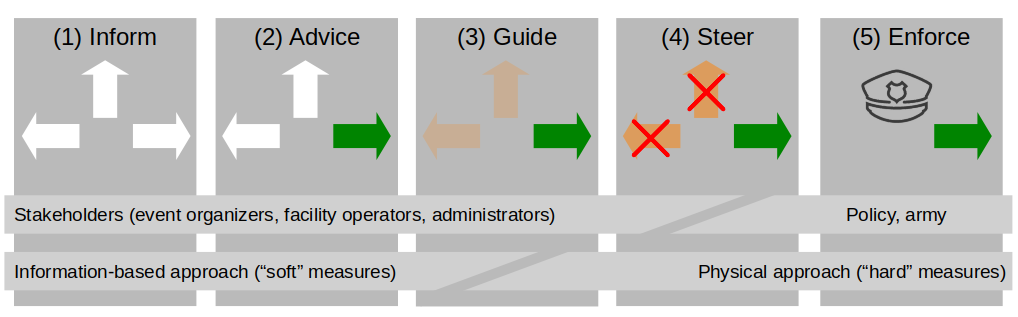
\includegraphics[width=\textwidth]{../figures/state-of-the-art/crowdmanagement/ficestages.png} 
\caption[Strategies for influencing crowd behavior ]{Strategies for influencing crowd behavior. Crowd management uses information-based approaches such as informing and providing advice (1,2). Crowd control employs physical measures to enforce a certain behavior (4,5). Guiding people (3) is located at the transition between the soft (1,2) and the hard (4,5) measures. Own graphic  inspired by \cite[p.168]{feliciani-2021-cdyn}. }
\label{fig:fivestages}
\end{figure}




In the `inform' stage, neutral information is provided using signs, maps, and colored paths. In the `advice' stage, information is manipulated to bias the decision, for example, the naming of walking paths: football fans might favor a walking path to the stadium named after a famous football player. Notably, the crowd is unaware of the manipulation~\cite[p.169]{feliciani-2021-cdyn}. 
In the `guiding' stage, the manipulation is presented obviously to the crowd using instructions that are disseminated through loudspeakers, announcements, information monitors, or light signage.  
The intensity of the measures is higher than in the `advice' stage and can involve low-intense physical measures such as staff blocking a closed gate. The crowd is fully aware of the manipulation.
In the `steer' stage physical measures, like for example placing a barrier, are employed. In this stage, it takes people great effort to defy the measures. In the `enforce' stage, specific behavior is enforced by the police or army using water cannons, tear gas, or brute force. Crowd management corresponds to the stages that aim to inform, advise, and guide~\cite{feliciani-2021-cdyn}. Importantly, people are free to decide whether to follow instructions. Therefore, it is essential to consider the compliance of people when developing a crowd guidance system.





\subsection{Quantitative characteristics of crowds and safety evaluation }
\label{sec:fundamentaldiagram}
 
Crowd and pedestrian behavior can be quantified and evaluated using several measurement quantities and metrics. One of them is the fundamental diagram that describes the relationship between density and flow~\cite{adrian-2019-cdyn}, see Fig.~\ref{fig:fundamental}. The flow increases over the density until the critical density is reached, at which the flow is maximal, that is, the capacity. Beyond the critical density, the flow decreases until the jamming density is reached, and movement is no longer possible.
The density range between $0\,\text{ped/m}^2$ and the critical density is called the free flow regime because there is enough space to allow most pedestrians to walk at their desired speeds~\cite{feliciani-2021-cdyn}. According to the Handbook of Fire Protection Engineering (SFPE)~\cite{hurley-2016-cdyn}, the free flow regime corresponds to a density range $[0\,\text{ped/m}^2, 1.88\,\text{ped/m}^2]$. 


\begin{figure}[hbt!]
\begin{tikzpicture}
\node[] at (0,0) {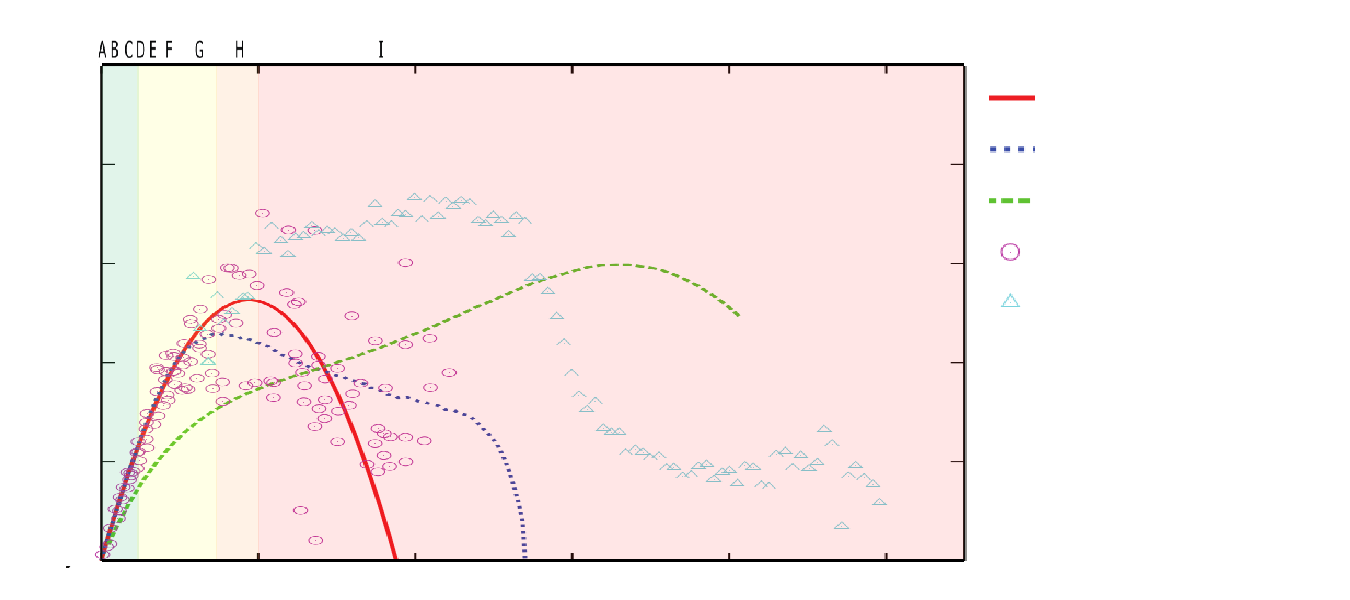
\includegraphics[width=15cm]{../figures/state-of-the-art/crowdmanagement/fundamental_diagram.pdf} };
\node[text width=5cm] at (6.8,2.2) {SFPE~\cite{hurley-2016-cdyn}};
\node[text width=5cm] at (6.8,1.6) {Weidmann~\cite{weidmann-1994-cdyn}};
\node[text width=5cm] at (6.8,1.1) {Predtechenskii~\cite{predtechenskii-1968-cdyn} };
\node[text width=5cm] at (6.8,0.6) {S. Older~\cite{older-1968-cdyn}};
\node[text width=5cm] at (6.8,0.0) { Helbing et al.~\cite{helbing-2007-cdyn} };

\node[text width=5cm] at (-0.8,-3.5) { Crowd density in $peds/m^2$};
\node[text width=5cm,rotate=90] at (-7.2,0.4) { Specific flow in $ped/(ms)$};
\node[text width=8cm] at (1.5,2.8) {  \begin{scriptsize} Level of Service according to Weidmann\end{scriptsize} };

\node[text width=5cm] at (-2,2.2) { Congestion};
\draw[->] (-4.6,1.9) -- (-3.7,1.9);
\draw[dashed] (-4.6,-3) -- (-4.6,2.1);

\node[] at (-6.2,-3.2) { \begin{footnotesize} 0 \end{footnotesize} };
\node[] at (-4.6,-3.2) { \begin{footnotesize} 2 \end{footnotesize} };
\node[] at (-2.9,-3.2) { \begin{footnotesize} 4 \end{footnotesize} };
\node[] at (-1.1,-3.2) { \begin{footnotesize} 6 \end{footnotesize} };
\node[] at (0.6,-3.2) { \begin{footnotesize} 8 \end{footnotesize} };
\node[] at (2.3,-3.2) { \begin{footnotesize} 10 \end{footnotesize} };

\node[] at (-6.7,-2.9) { \begin{footnotesize} 0 \end{footnotesize} };
\node[] at (-6.7,-0.7) { \begin{footnotesize} 1 \end{footnotesize} };
\node[] at (-6.7,1.5) { \begin{footnotesize} 2 \end{footnotesize} };



\end{tikzpicture}
\caption{Fundamental diagram. The flow increases over the density until the maximum flow (capacity) is reached. For higher densities, the flow decreases. The shape of the fundamental diagram differs for the studies~\cite{hurley-2016-cdyn,weidmann-1994-cdyn,predtechenskii-1968-cdyn,older-1968-cdyn,helbing-2007-cdyn} because it depends on several factors, such as age or culture. Own graphic inspired by~\cite{zhang-2012e-cdyn,kitzlinger-2020-cdyn}.}
\label{fig:fundamental}
\end{figure}


As one can observe in Fig.~\ref{fig:fundamental}, the fundamental diagram differs from study because the density-flow-relationship depends on several factors: topological features, such as crossings, stairs~\cite{burghardt-2013-cdyn}, the directionality of flows~\cite{feliciani-2016b-cdyn}, age~\cite{cao-2016-cdyn,ren-2019-cdyn}, religion~\cite{subramanian-2021-cdyn}, and culture~\cite{chattaraj-2009-cdyn}, visibility conditions~\cite{cao-2018-cdyn}, the motivational level~\cite{ye-2012-cdyn}, environmental conditions such as the temperature~\cite{kim-2018-cdyn}, and the measurement method~\cite{zhang-2012e-cdyn}. For an overview of factors, I refer to~\cite{paetzke-2023-cdyn}.

Important for crowd management applications is that the location and size of the measurement area have an influence:  The maximum density cannot be measured in the center of a bottleneck but in front of it~\cite{zhang-2012e-cdyn}. Also, the larger the area, the smoother the density measurements.



To describe the relationship between flow and density analytically, numerous models have been proposed, see e.g.~\cite{hurley-2016-cdyn,mori-1987-cdyn,bosina-2018-cdyn,fruin-1971-cdyn,lam-1995-cdyn,navin-1969-cdyn}. In the pedestrian dynamics community, the Kladec equation~\cite{weidmann-1992-cdyn} is widely used that relates the specific flow $J_s$ to the density $\rho$:
\begin{equation}
J_s = \rho v_0  \left( 1  - e^{-1.913 \left(  \frac{1}{\rho} - \frac{1}{\rho_{\text{jam}}} \right) }  \right)
\label{eq:kladec}
\end{equation}
with the jamming density $\rho_\text{jam}=5.4\,\text{ped/m}^2$ and the free flow velocity $v_0=1.34\,\text{m/s}$ according to Weidmann~\cite{weidmann-1992-cdyn}.


\subsubsection{Congestion definition based on the fundamental diagram}
The definition of congestion is an ongoing topic within the pedestrian dynamics community. Currently, no standardized definition is available. Compare, for example, the definitions in~\cite{rimea-2016-cdyn} and~\cite{kitzlinger-2020-cdyn}.
Kitzlinger et al.~\cite{kitzlinger-2020-cdyn} suggest defining congestion based on the fundamental diagram: Congestion is present when the capacity is exceeded, or, in terms of flows, jamming occurs if the inflow is larger than the capacity. This criterion is identical to the jamming criterion proposed in~\cite{schadschneider-2009-cdyn,zhang-2011-cdyn}. 
In terms of densities, this means that the density must stay below the critical density.

There are several values suggested for the critical density: $1.75\,\text{ped/m}^2$ according to Weidmann~\cite{weidmann-1994-cdyn}, $2.16\,\text{ped/m}^2$ according to Fruin~\cite{fruin-1971-cdyn}, $1.88\,\text{ped/m}^2$ according to the Handbook of Fire Protection Engineering~\cite{hurley-2016-cdyn} and $6.64\,\text{ped/m}^2$ according to Predtechenskii~\cite{predtechenskii-1968-cdyn}. Except from the study in~\cite{predtechenskii-1968-cdyn}, the critical density is always around $2\,\text{ped/m}^2$ which aligns with the qualitative observations of Oberhagemann~\cite{oberhagemann-2012-cdyn}. Therefore, this value is a suitable threshold for crowd management applications.

\subsubsection{Level of service: Basis for safety evaluation}

The Level of Service (LOS) qualitatively describes the movement behavior of a crowd. The density is divided into levels, each qualitatively describing a certain movement behavior, see Tab.~\ref{tab:levelofservice}. Therefore, it is used to evaluate safety and comfort. 

Like the fundamental diagram, the qualitative movement behavior depends on numerous factors, which is why different level of service schemes have been proposed~\cite{yadav-2024-cdyn}. In crowd management applications, the categorizations according to Fruin~\cite{fruin-1971-cdyn} and Weidmann~\cite{weidmann-1994-cdyn} are typically used, see~Fig.~\ref{fig:fruinweidmann}. 



\begin{table}[hbt!]
\centering
Level of Service according to Fruin~\cite{fruin-1971-cdyn}
\begin{tabular}{p{1.0cm}p{8.5cm}p{1.5cm}p{1.5cm}}
\hline 
Level  & Walking behavior &Density $\text{ped/m}^2$ & Flow $\text{ped/m/min}$  \\ 
\hline
A & Pedestrians walk with their desired speed &  $<0.31$ & $<23.0$  \\ 
B & Occasionally interference with other pedestrians & $<0.43$ & $<30.5$ \\ 
C & Partially reduced walking speed & $<0.72$ & $<49.2$   \\ 
D & Rare passing maneuvers & $<1.08$ & $<65.6$  \\ 
E &Temporal stops, no passing maneuvers     & $<2.17$ & $<82.0$  \\ 
F &Physical contact between crowd members  &  $\geq 2.17$ & $ \geq 82.0$   \\ 
\hline 
\end{tabular} 
\caption[Level-of-Service concept for pedestrian traffic]{Level-of-Service levels for pedestrian traffic according to Fruin~\cite{fruin-1971-cdyn}. Density and flow values are only valid for walkways. The best category is the A level, where the density and flow are the lowest.}
\label{tab:levelofservice}
\end{table}



\begin{figure}[hbt!]
\centering
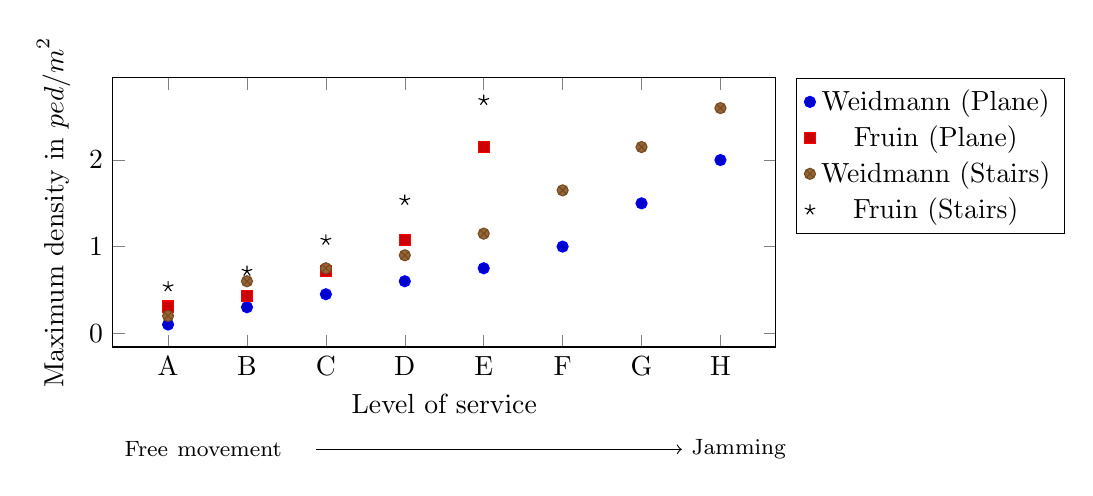
\begin{tikzpicture}
\begin{axis}[xlabel=Level of service,legend entries={Weidmann (Plane), Fruin (Plane),  Weidmann (Stairs), Fruin (Stairs)}, legend pos=outer north east, ylabel={Maximum density in $\text{ped/m}^2$},width=10cm,height=5cm, xtick={1,2,3,4,5,6,7,8}, 
  xticklabels={A,B,C,D,E,F,G,H},]
\addplot+ [only marks] table [] {
x y
1 0.1
2 0.3
3 0.45
4 0.6
5 0.75
6 1.0
7 1.5
8 2.0
};
\addplot+ [only marks] table [y expr=10.7639150512/\thisrow{y}] {
x y
1 35
2 25
3 15
4 10
5 5 Oberhagemann \cite{oberhagemann-2012-cdyn} haben Einteilungen vorgeschlagen.

};
\addplot+ [only marks] table [] {
x y
1 0.2
2 0.6
3 0.75
4 0.9
5 1.15
6 1.65
7 2.15
8 2.6
};
\addplot+ [only marks] table [y expr=10.7639150512/\thisrow{y}] {
x y
1 20
2 15
3 10
4 7
5 4
};
\end{axis}
\node[text width=2.3cm] (a) at (1.3,-1.3) {\begin{footnotesize}Free movement\end{footnotesize}};
\node[text width=2.3cm] (c) at (8.5,-1.3) {\begin{footnotesize}Jamming \end{footnotesize}};
\draw[->] (a) -- (c);

\end{tikzpicture}
\caption{Upper density bounds of the Level-of-Service concepts according to Weidmann~\cite{weidmann-1994-cdyn} and Fruin~\cite{fruin-1971-cdyn}. For each level the maximum density is depicted for walkways (`Plane') and stairs. The higher the level, the stronger the maximum densities differ (A is the lowest level). One can observe that Weidmann's classification~\cite{weidmann-1994-cdyn} is more rigorous than Fruin's~\cite{fruin-1971-cdyn}: The blue and brown data points are always below the red and black data points.  }
\label{fig:fruinweidmann}
\end{figure}

Weidmann~\cite{weidmann-1994-cdyn} divides the density into nine levels depending on the traffic situation, assigning them levels A (best level) to I (worst level). Free movement in the plane is present at densities $<0.1\,\text{ped/m}^2$, which corresponds to level A~\cite[p.97]{weidmann-1994-cdyn}. In Level I, the density $>2\,\text{ped/m}^2$ which means there is 'massive crowding'~\cite[p.97]{weidmann-1994-cdyn}. 

Fruin distinguishes only six levels: A-F. The A level describes a free-flow situation, while the F level describes a standstill situation, see Tab.~\ref{tab:levelofservice}. Like Weidmann~\cite{weidmann-1994-cdyn}, Fruin~\cite{fruin-1971-cdyn} adjusts the density and flow intervals depending on the scenario. For walking in the plane and for stairs, the density maximal density for each level differs strongly, see again Fig.~\ref{fig:fruinweidmann}. 

\subsubsection{Evaluation of safety and comfort}
\label{sec:risk}

Safety and comfort are evaluated using flow or density-based criteria. Several recommendations are available that are based on the level of service concept: Weidmann~\cite{weidmann-1994-cdyn} recommends a B level for walkways in general. A level D is only acceptable during the rush hour  and a level F is acceptable in bottlenecks where people do not stay a long time~\cite{weidmann-1994-cdyn}. The Highway Capacity Manual~\cite{hpc-2022-cdyn} provide recommendations based on the level of service concept according to Fruin~\cite{fruin-1971-cdyn}: at least a level E should be achieved which is similar to the jamming criterion.

The Pedestrian Comfort Level~\cite{tfl-2019-cdyn} is a flow-based metric for evaluating comfort.
The recommended level depends on the scenario because it is assumed that pedestrians' perception is scenario-specific. In tourist areas where people are likely to spend time voluntarily, people might be particularly sensitive to crowding. In this case, a maximum flow of $11\,\text{ped/min/m}$ is recommended. For a transfer scenario at a train station where commuters stay just a short time, a flow of  $17\,\text{ped/min/m}$ is acceptable, see Fig.~\ref{fig:pedcomfortlevel}.




\begin{figure}[hbt!]
\centering
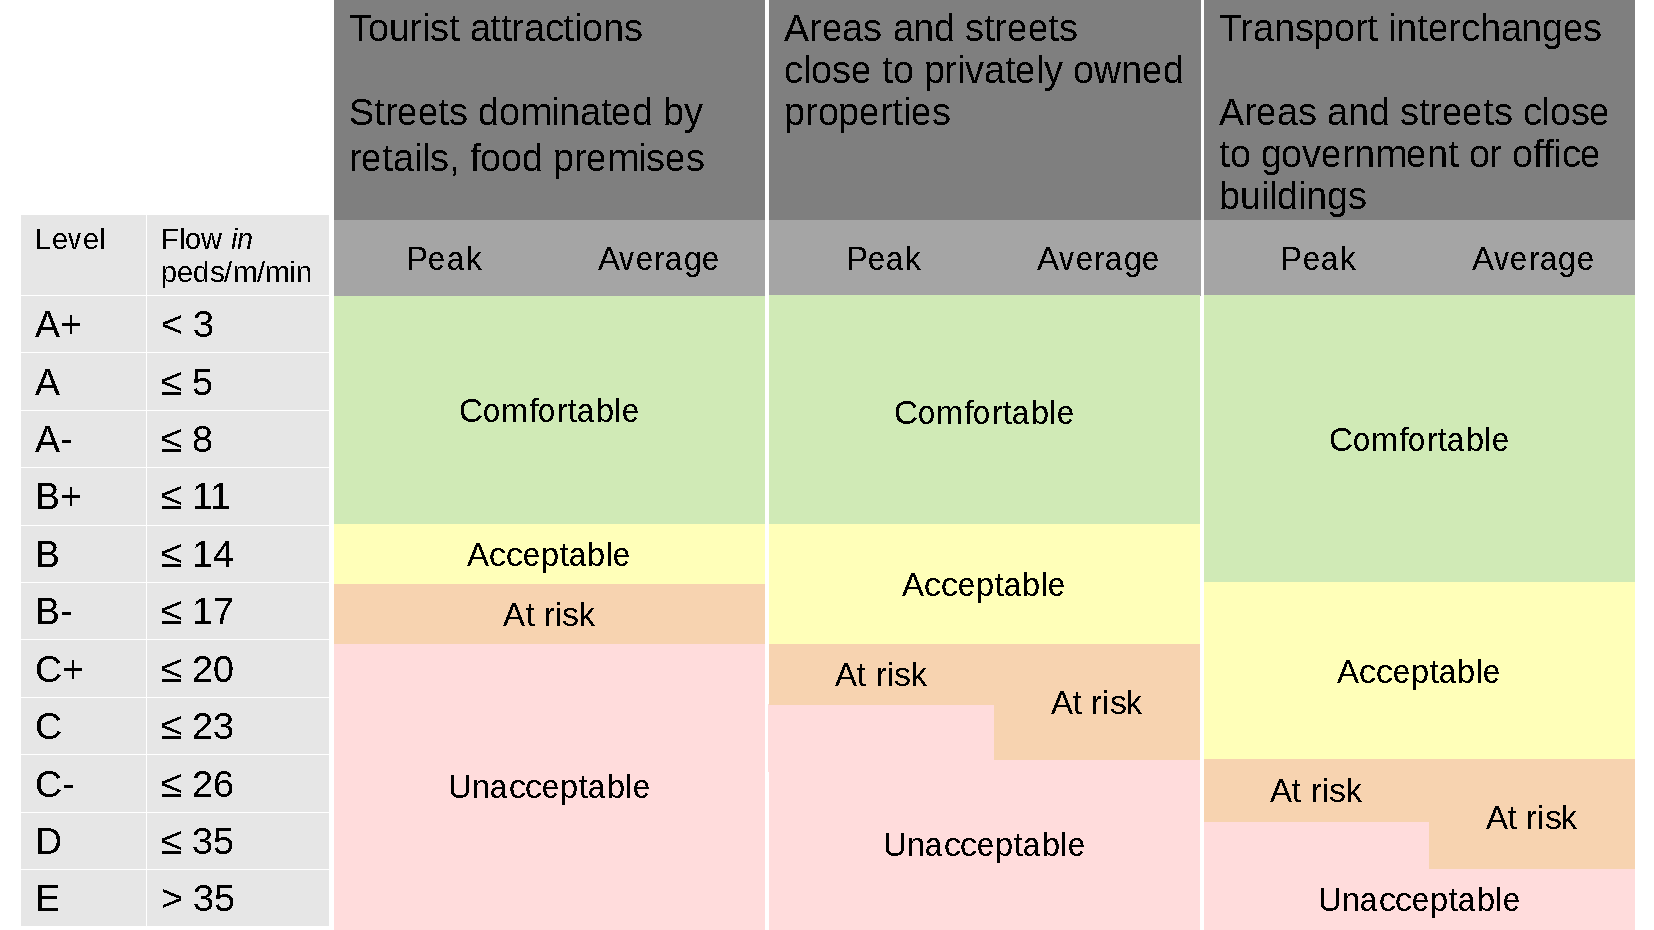
\includegraphics[width=12.5cm]{../figures/state-of-the-art/crowdmanagement/pcl.pdf} 
\caption[Pedestrian Comfort Levels for different traffic scenarios]{Pedestrian Comfort Levels for different traffic scenarios. It is assumed that people experience comfort scenario-specifically: They are more sensitive to crowding in tourist areas, where they spend their spare time, than at train stations where they only pass a short time for traveling. Own graphic based on the recommendations from~\cite{tfl-2019-cdyn}.}
\label{fig:pedcomfortlevel}
\end{figure}



Finally, I would like to address so-called safety indices~\cite{carter-2007-cdyn,zegeer-2006-cdyn,montella-2020-cdyn,krishnan-2023-cdyn}, as I have repeatedly come across these metrics in my literature research.
Safety indices are used in traffic engineering to compare traffic scenarios within a city. With this, a traffic engineer can identify the most safety-critical spots for improving traffic. However, these indices are unsuitable for crowd management because they only compare but do not evaluate safety. 



\subsection{Key theories on crowd behaviour}
\label{sec:crowdbah}


A prerequisite for the development of crowd management applications is understanding crowds' behavior. 
Several theories have been proposed to explain the psychological behavior of crowds~\cite{lebon-1895-life,freud-1921-life,allport-1924-life,zimbardo-1999-life,sherif-1936-life,turner-1957-life,berk-1974-life,berk-1974a-life}. One can distinguish between classical and modern theories. Classical theories only explain violent behavior but cannot explain peaceful gatherings, so these theories are regarded as outdated~\cite{challenger-2009-cdyn}. Since modern theories have emerged from these, I find it essential to be familiar with their basic principles, so I briefly list the key ideas in Tab~\ref{tab:classicaltheories}.



\begin{table}[hbt!]
\begin{tabular}{p{4cm}p{10cm}}
 \hline
Classical theory & Basic idea \\ \hline
Le Bon's Group Mind Theory (1895)  \cite{lebon-1895-life} & Individuals lose their sense of self in a crowd and become anonymous. The actions of the crowd are driven by a group mind controlled by primitive instincts. Therefore, crowds are disruptive by nature.  \\ 
Theory according to Freud (1921)  \cite{freud-1921-life} & Individuals' super-ego is surpassed when they are in a crowd which unlocks their unconscious mind. Therefore, individuals are driven by their instincts.  \\
 Individualism Theory (1924)  \cite{allport-1924-life} & Crowd violence is caused by violent predispositions of individuals. Predispositioned individuals reinforce each others' behavior, which aggregates violent behavior. \\
 Deindividuation Theory (1952-1989)  \cite{zimbardo-1999-life} & The anonymity of the crowd members controls the behavior. Individuals lose their self-awareness. The resulting anonymity causes antisocial behaviors.\\
 \hline
\end{tabular}
\caption{Classical theories on crowd behavior. These theories explain violent behavior of crowds but cannot explain peaceful gatherings.   }
\label{tab:classicaltheories}
\end{table}

\subsubsection{Modern crowd theories}

Modern crowd theories aim to explain crowd behavior more generally than classical theories.
The \textit{Theory of Social Norms} (1936)~\cite{sherif-1936-life} introduces the concept of social norms. \enquote{When a group of individuals faces a new unstable situation
and has no previously established interests or opinions regarding the situation, the result is not chaos; a common norm arises, and the situation is structured in relation to the
common norm}~\cite[p.111]{sherif-1936-life}. 
%
The \textit{Emergent Norm Theory} (1957-1964)~\cite{turner-1957-life} extends the concept of social norms. Through interactions, individuals develop new behavioral norms.
%
The \textit{Game Theory} (1972-1974)~\cite{berk-1974-life,berk-1974a-life} assumes that crowds act rationally. Individuals perform actions they believe bring the highest payoff. Crowd members seek information from which they predict possible events. Depending on the reward, the actions are derived, starting with the action that maximizes the reward. Since the reward is difficult to determine in advance, the theory lacks of applicability.
%
The \textit{Place Scripts Theory} (1992)~\cite{donald-1992-life} suggests that individuals follow behavioral patterns. The sequence of actions is called the script. Each action is associated with a certain place. \enquote{They define, understand, or formulate a script in relation to where they are and interpret the behavior of others.}~\cite{donald-1992-life}. According to the theory, familiarity with the environment is disadvantageous in emergency situations, which might not be always the case in reality. %
The \textit{Self-categorization Theory} explains how individuals view themselves in relation to other individuals as a group and how the view of an individual changes when they become a group member. It is based on the meta-contrast principle: Group members perceive strong similarities between themselves and other group members and large differences between themselves and non-group members~\cite{turner-1994-life}.
The \textit{Social Identity Theory}~\cite{tajfel-1974-life,tajfel-1979-life,tajfel-1982b-life,turner-1972-life,turner-1981-life,turner-1982-life,turner-1987c-life} explains how an individual's behavior is influenced by a social identity to a group or crowd, which in turn influences collective behavior. The extent of the sense of belonging is also referred to as the degree of social identification~\cite{templeton-2020-life}. An example is a group of football fans who identify themselves as football fans. The assumption is that exactly one of a person's social identities is salient at a time: For the football fan only the fan identity is salient. Other identities such as being an academic or a painter do not have an effect.

The \textit{Social Identity approach} combines the self-categorization theory with the social identity theory~\cite{templeton-2020-life}.
It is supported by empirical evidence from numerous experiments that demonstrate the effect of social identities on decision-making and movement behavior. 
In-group members who share a social identity are more strongly influenced by members of their social group (in-group members) than by non-group members~\cite{levine-2005-life,carter-2015-life,reicher-2016-life,sivers-2014b-cdyn}. Non-group members are members of an opposing social group, e.g., football fans of the opposing team or people whose group membership is unknown. Sharing a social identity affects the behavior: It was observed that people are more likely to help each other when sharing a social identity~\cite{levine-2005-life}. Consequently, social identities can reinforce positive characteristics and behavior.  Negative emotional responses become weaker: One example is that less disgust is perceived within a group compared to non-group members~\cite{reicher-2016-life}. Social identities also influence mobility behavior. Group members tolerate dense situations more likely and might even enjoy  staying in denser and more central parts of the crowd~\cite{novelli-2013-life}. They also move slower than individuals and stay closer together~\cite{templeton-2018-cdyn}. 
Also, different formations have been observed for groups:  walking next to each other, walking in line, or forming a V-shape~\cite{gorrini-2014-cdyn, koster-2011b-cdyn, moussaid-2010-cdyn, qiu-2010-cdyn,subramanian-2022-cdyn}. 

\subsubsection{Communication with crowds}


For the categorization of communication strategies, a basic understanding of the elements of the communication process is necessary. Therefore, I briefly introduce Berlo's communication model~\cite{berlo-1960-life} which focuses on the components of the communication process. I used them as categories in my literature research. 

Berlo's model~\cite{berlo-1960-life} is composed of a sender, a message, a channel, and a receiver, see Fig.~\ref{fig:commmodel}. 
Senders encode their thoughts into a message that is transmitted over a communication channel. The receiver perceives the message and decodes the information. Several factors, such as the socio-cultural background, the structure and content of a message, or the channel, influence the communication process. Studies in the field of crowd management mainly focus on the channel, testing the suitability of instructions from personnel~\cite{feliciani-2020b-cdyn}, background music~\cite{zeng-2019-cdyn}, or auxiliary equipment, such as robots~\cite{zhou-2019-cdyn}, for the provision of information. There is scarcely any research on employing mobile applications and smartphones for guiding crowds except for one experiment in which a crowd received instructions via their smartphones to accelerate evacuation from a room with four exits~\cite{feliciani-2020-cdyn}.







\begin{figure}[hbt!]
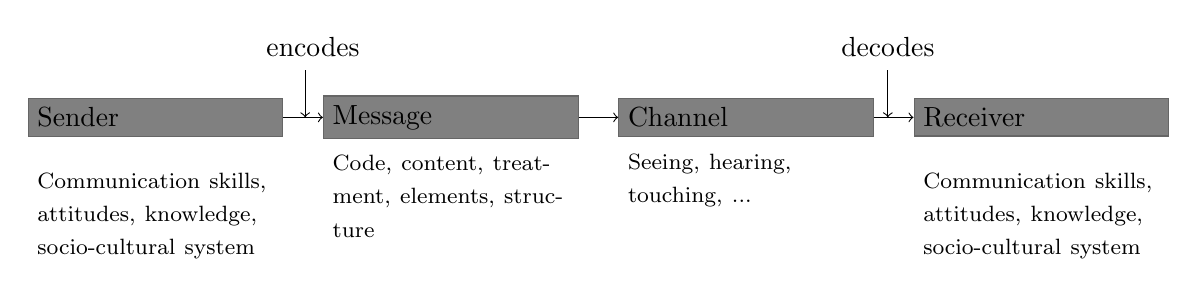
\begin{tikzpicture}

\node[rectangle,draw=black!60,fill=gray,text width=3.0cm] (a) at (0,0.0)                            { Sender };
\node[rectangle,draw=black!60,fill=gray,text width=3.0cm] (b) at (3.75,0.0)                            {Message };
\node[rectangle,draw=black!60,fill=gray,text width=3.0cm] (c) at (7.5,0.0)                            {Channel };
\node[rectangle,draw=black!60,fill=gray,text width=3.0cm] (d) at (11.25,0.0)                            {Receiver };
\draw[->] (a) -- (b);
\draw[->] (b) -- (c);
\draw[->] (c) -- (d);

\draw[->] (1.9,0.6) -- (1.9,0);
\node at (2,0.9) {encodes};

\draw[->] (9.3,0.6) -- (9.3,0);
\node at (9.3,0.9) {decodes};

\node[text width=3.0cm] (a) at (0,-1.25)                            { 
\begin{footnotesize}Communication skills,
attitudes, knowledge, socio-cultural system
\end{footnotesize}
 };
\node[text width=3.0cm] (b) at (3.75,-1.0)                            {\begin{footnotesize}Code, content, treatment, elements, structure
\end{footnotesize} };
\node[text width=3.0cm] (c) at (7.5,-0.8)                            {\begin{footnotesize}Seeing, hearing, touching, ... \end{footnotesize} };
\node[text width=3.0cm] (d) at (11.25,-1.25)                            {\begin{footnotesize}Communication skills,
attitudes, knowledge, socio-cultural system
\end{footnotesize} };

\end{tikzpicture}
\caption{ Components and factors of the communication process. Own graphic of Berlo's communication model proposed in~\cite{berlo-1960-life}.}
\label{fig:commmodel}
\end{figure}


Numerous theories and experimental studies aim to understand how information can be efficiently communicated to crowds in emergencies.  Reynolds et al.~\cite{reynolds-2005-life} provide a theoretical basis by introducing the Crisis and Emergency Risk Communication Model that defines communication activities for different phases of a disaster. 
Drury et al.~\cite{drury-2009-life} conducted a virtual reality experiment where participants imagined being at a metro station when a fire breaks out. They found that people helped each other more often when they shared a social identity. 


Reicher et al.~\cite[p.16]{reicher-2004-life} stress the necessity of communication in conflicts: \enquote{[...] it becomes increasingly important to communicate with the crowd where one seeks to avoid a potentially conflictual relationship, but in situations where relationships are potentially conflictual, crowd members are least likely to trust what the police have to say}. 
Also, it is suggested to use mediators that are trusted and respected within the crowd~\cite{reicher-2004-life}. 
Other studies focus on the design of signage that assesses where and how signs should be placed~\cite{farr-2012-life}. 

Palttala et al.~\cite{palttala-2012-cdyn} suggest employing several communication strategies at once to address heterogeneous crowds.
Van der Wal et al.~\cite{wal-2021-life} found that "dynamic emergency exit floor lighting and staff guiding people to exits were only beneficial for high-density crowds and those unfamiliar with the environment". 
%

Numerous studies from the communication sciences investigate how the message content affects decision behavior. In particular, the quantity and quality of information are analyzed: how much information is necessary? In which way should a particular piece of information be presented? The latter includes the so-called message framing, i.e., `presenting logically equivalent options in semantically different ways'~\cite{krishnamurthy-2001-life}.
%
Message framing plays a role in numerous fields of application. 
In some studies, message framing did not have any effect: Carfora et al.~\cite{carfora-2022b-life} found that the message components `..., you will feel more energetic' and  `..., you will feel less tired' were equally effective in persuading people to switch to a particular diet. Capps at al.~\cite{capps-2022-life} tested the effect of message framing on sanitizer usage during the Covid-19 pandemic. They put different signage next to sanitizers with three different messages: (1) `Using hand sanitizer means you're doing your part to fight the spread of COVID-19 ... Stay healthy!', (2) `Many people use hand sanitizer to fight the spread of COVID-19 ... Join them!', and (3) `More and more people are using hand sanitizer to fight the spread of COVID-19 ... Join them!'. They could not find a statistical difference in sanitizer usage. 

Other studies provide strong evidence that message framing indeed affects the behavior: Nobel~\cite{nobel-2022-life} investigated how message framing can affect peoples' decision to quit smoking. He found that messages that emphasize the financial gain from cigarette cost savings are more effective than loss-oriented messages, such as `if you continue to smoke, you will lose money'. Moreover, he found that addressing the financial advantage is more effective than addressing health aspects such as longevity `if you quit smoking, you will live longer'.
%
In some of the studies the amount of information and number of instructions was varied: Carter et al.~\cite{carter-2014-life,carter-2015-life} conducted studies on mass decontamination and found that the highest level of compliance was achieved when the public was provided with both health-focused information and practical information.
Osman et al.~\cite{osman-2018-life} found that health-related information about smoking increases the tendency to advocate regulations on smoking.
Several other studies exist in which message framing was tested for a particular purpose, see the overview in~\cite{gallagher-2012-life}. 

The examples from my literature research show that message framing can indeed influence behavior of individuals and crowds. 
However, it depends on the use case and the wording whether message framing is particularly effective. It is unclear how message framing can be employed via mobile applications in a crowd guidance system. 
It is, therefore, necessary to investigate how redirection recommendations should be phrased to foster compliance.











\subsection{Pedestrian and crowd sensing technologies}

Crowd-sensing is the task of measuring at least one crowd characteristic~\cite{teixeira-2010-cdyn}:
\begin{itemize}
\item Presence: Is someone present?
\item Count: How many people are present? 
\item Location: How are pedestrians distributed in a space?
\item Track: How do pedestrians move?
\item Identity: Who are the pedestrians?
\end{itemize}


\subsubsection{Visualization-based approaches}
Several technologies are available to detect, count, track, and monitor pedestrians and crowds.
\enquote{One of the most commonly employed solutions to count, track, and analyze pedestrian
activity in public spaces is the use of images from (surveillance) cameras}~\cite[p.79]{feliciani-2021-cdyn}. Optical cameras, thermal cameras, and LiDar-based systems are categorized as visualization-based technologies. All visualization-based approaches have in common that crowd characteristics are derived from image data for which computer vision or machine learning techniques are used, see Tab.~\ref{tab:verfahrenbildinfo}.
 
 
\begin{table}[hbt!]
\centering
\begin{tabular}{llll}
\hline 
Image descriptors & Classifiers \\ \hline
Histogram of oriented gradients &  Support vector machines \\ %& pixel-based procedure that divides the image into cells and estimates gradient directions and edge orientations, used for object detection \\ 
Local Binary Pattern  & Neuronal Networks  \\ % classifier, used in combination with the Histogram of oriented gradients descriptor \\
Haar-like feature  & Gaussian (Mixture) Model \\ %uses Haar wavelet representations for face recognition; does not consider motion  \\
Viola-Jones feature & ... \\
... &  \\ % & uses Haar wavelets and particle filters for dynamic face recognition \\
%& Discriminative deep model based on Restricted Boltzmann Machine (RBM) building blocks  & \\
 \hline
\end{tabular} 
\caption{Examples of image descriptors and classifiers used to gain information about a crowd from images. Application examples can be found in~\cite{brunetti-2018-cdyn}.}
\label{tab:verfahrenbildinfo}
\end{table} 




\subsubsection{Non visualization-based approaches}
Non-visualization-based technologies estimate crowd properties by using radio signals, temperature, or sounds, see Fig.~\ref{fig:classification}. The approaches can be classified as device-free or device-based.


\begin{figure}[hbt!]
\centering
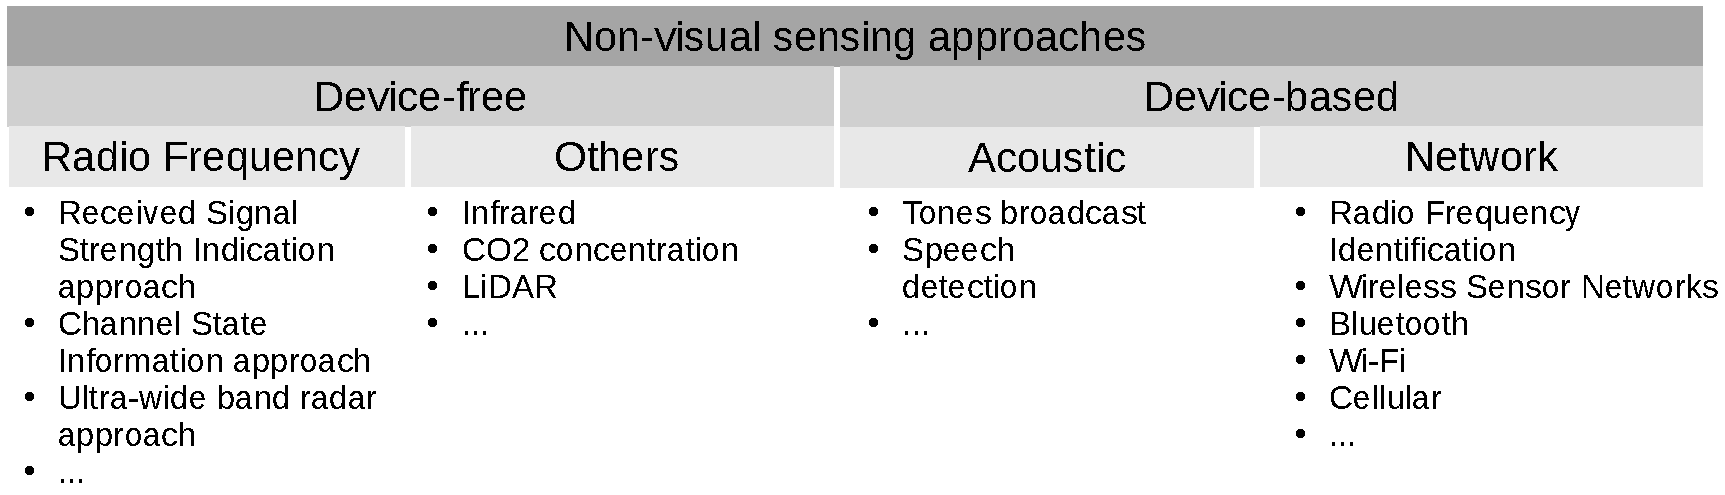
\includegraphics[width=0.9\textwidth]{../figures/state-of-the-art/crowdmanagement/sensing_nonvisual.pdf} 
\caption[]{Categorization of non-visualization-based sensing technologies. Own \mbox{graphics} inspired by~\cite{kouyoumdjieva-2019-cdyn}.  }
\label{fig:classification}
\end{figure}
%



Device-free approaches do not require crowd members to carry special sensors or devices~\cite{kouyoumdjieva-2019-cdyn}. Some of these device-free approaches employ the radio frequency band. In the \textit{Received Signal Strength Indication} approach, the sensor measures the power of a radio signal of a known radio infrastructure node such as WLAN access point. Since pedestrians hinder wave propagation, it is assumed that the number of pedestrians is high when the power is low and vice versa. The same principle is used in the \textit{Channel State Information} approach. Here, however, signals are transmitted on multiple frequencies (OFDM), which allows the power level and, thus, the number of people to be determined more precisely~\cite{wu-2012-com}.
So-called \textit{ultra-wide band} radar sensors also work with radio frequencies. They estimate the number of people by emitting an impulse signal and analyzing its reflection~\cite{choi-2017-com}. 
%
Some other approaches do not use the radio band. These include \textit{infrared} sensors, which correspond to the industry standard among device-free methods~\cite{kouyoumdjieva-2019-cdyn}. They either detect the body temperature (pyroelectric infrared sensor) or act as a light barrier: when the light beam is interrupted, the count is increased. Although simultaneous crossings are not recognized, the number of people is only underestimated by 10\% on average~\cite{olivo-2019-cdyn}. Some procedures estimate the number of people based on the CO2 concentration in a room~\cite{lei-2021-cdyn}. Others are based on LiDAR or use a combination of technologies (see e.g.~\cite{leykin-2010-cdyn}).
An overview of device-free approaches can be found in~\cite{kouyoumdjieva-2019-cdyn}.






Device-based approaches require people to carry a sensor or device that is recognized~\cite{kouyoumdjieva-2019-cdyn}. Therefore, the accuracy depends on the participation. To tackle this, a procedure to estimate the participation has been proposed, see~\cite{nicolai-2007-com}. Unfortunately it is based on collected data and cannot measure the current participation. Most device-based approaches use network technologies to count people. 
Technologies employing Radio Frequency Identification (RFID) require that the crowd members carry RFID tags. Hidayat et al.~\cite{hidayat-2019-com} propose an RFID-based system for tracking pilgrims during the Hajj festival. Another technology is Near Field Communication (NFC). A device with NFC functionalities sends a signal to the reader if they get in proximity. Bluetooth-based technologies employ the same principle.  
Weppner et al. ~\cite{weppner-2014-com} installed Bluetooth scanners at a bridge to detect spectators in Zurich, Switzerland. They found that the motion pattern of the crowd can be determined from a small number of mobile nodes. Versichele et al.~\cite{versichele-2012-com} used Bluetooth to estimate the spatio-temporal distribution of a crowd at a festival. Den Heuvel et al.~\cite{heuvel-2015-cdyn} use Bluetooth scanners to investigate route choice behavior and waiting time at stairs and escalators at Utrecht Central Station (Netherlands).


Another device-based approach is based on WiFi: At a WiFi Access Point the number of Medium Access Control (MAC) addresses is counted. It is assumed that each count is one pedestrian. Such systems are in operation at Amsterdam Airport Schiphol\footnote{Amsterdam Airport Schiphol. Royal Schiphol Group Privacy Statement. Available online: \url{https://www.schiphol.nl/en/privacy-policy/} (accessed on 13 Jan 2024) } and in public transport stations in
London\footnote{Transport for London. Review of the TfL WiFi Pilot. Available online: \url{http://content.tfl.gov.uk/review-tfl-wifi-pilot.pdf}. (accessed on 12 February 2019).}.
However, the estimates have become inaccurate after procedures were introduced that randomize the medium access control addresses regularly. Active research tries to improve the accuracy~\cite{nitti-2020-com,vega-2021-com}. 
Other approaches rely on the cellular network.
Shibata et al.~\cite{shibata-2019-com} propose to estimate the crowd density from the signal strength of the uplinks from smartphones in an LTE network. Di Domenico et al.~\cite{domenico-2017-com} propose a procedure similar to the concept that is already applied in device-free approaches: They estimate the number of pedestrians based on fluctuations of signals. There is also an approach suggested that is based on direct communication: UrbanCount~\cite{danielis-2017-com} is a high layer protocol that has been proposed to estimate the total number of pedestrians in an area. It does not require a certain technology and has not been implemented in practice so far. It is unclear whether the protocol can identify crowd congestion.



\subsubsection{Range and accuracy}
Due to the different technologies, the range and accuracy of sensing approaches differ strongly, see Tab.~\ref{tab:technology_data}. Infrared sensors have the shortest range, except for near-field communication technologies and pressure sensors. Network-based technologies have a range of several hundred meters or even kilometers. However, these methods have the disadvantage that personal data is processed, which is why they are critical in terms of privacy in~\cite{darsena-2023-cdyn}. Direct communication technologies may not face this problem because  there is no intermediate processing data.


\begin{table}[hbt!]
\begin{footnotesize}
\begin{tabular}{p{45mm}p{25mm}p{10mm}p{12mm}p{10mm}p{10mm}p{10mm}p{10mm}}
 \hline
        Technology & Frequency & Max Range & User Cooper. & Accuracy & Privacy Issues\\
        \hline
        Optical camera & Visible & 100 m & No & High & Critical  \\ 
        Thermal camera & Infrared & 500 m  & No & High & Moderate\\
        LiDAR & Ultraviolet, Visible, Near Infrared & 1 km  & No & High & Moderate  \\
        Synthetic Aperture Radar & Ku/Ka band & 10 m  & No & High  & Moderate  \\ \hline
        (Passive) Infrared Sensor & Infrared & 10 m  & No & High & Low  \\
        Acoustic & 0.01-100 kHz & 20 m  & No & Low & Moderate \\
        Impulse-Radio Ultra-Wideband radar  & 3.1-10.6 GHz  & Low & No & High  & Low \\
        
        Radio Frequency Ident. & 13.56 MHz & 10 cm  & Yes & High & Critical \\
        Near Field Communication & 13.56 MHz & 10 cm  & Yes & High  & Critical  \\
        Bluetooth & 2.4 GHz & 50 m  & Yes & Medium  & Critical  \\
        WiFi & 2.4/5 GHz & 100 m  & Yes & Low & Critical \\
        LTE & 0.8/1.8/2.6 GHz & 10 km  & Yes  & High & Moderate \\
        5G & Sub-6 GHz & 10 km  & Yes & Low & Moderate  \\
        5G & MMW band & 1 km  & Yes & Medium & Moderate  \\
        Pressure & None & Contact  & Low & No   & Low  \\
        Received Signal Strength Indicator/Channel State Information  & Various & Variable  & No & Medium &  Low \\
        \hline
\end{tabular}
\end{footnotesize}
    \caption{Crowd sensing technologies. The upper part comprises visualization-based technologies like cameras. The lower part contains non-visualization-based technologies. The table data is based on the data presented in~\cite{darsena-2023-cdyn}.}
    \label{tab:technology_data}
\end{table}

My review of crowd-sensing approaches shows that there are several technologies for measuring crowd characteristics. 
Importantly, there is currently no sensing approach available that measures safety-critical crowd densities based on direct communication. I conclude that a novel approach is needed. 



\subsubsection{Detection of 'anomalies' and emotional states }
Novel sensing approaches aim to detect anomalous behavior and emotions in a crowd.  In~\cite{hassner-2012-cdyn}, the authors suggest using a support vector machine to identify violent behavior in a crowd from video footage from surveillance cameras. To measure the stress of spectators during a festival, Bergner~\cite{bergner-2020-cdyn} uses wristbands with sensors that measure accelerations, changes in skin conductivity and temperature, and GPS-trackers. Baig et al.~\cite{baig-2014-cdyn} suggest to infer emotions from motion behavior. Most approaches use machine learning to detect `anomalies' in the behavior of crowds: See the overviews in~\cite{sinha-2021-cdyn,lamba-2017-cdyn}. This is debatable since no standardized definition of anomaly exists: compare, e.g., \cite{mohammadi-2017-cdyn} and \cite{liu-2019-cdyn}. In my investigates, I will, therefore, rely on established metrics based on density and flows to assess the current state of the crowd.





\subsection{Suggested automatic crowd guidance systems}

\label{sec:modelalg}



I understand automatic guidance systems to automatically provide recommendations for pedestrian crowds. Advanced Traveller Information Systems, as proposed in~\cite{essen-2016-cdyn,sato-2014-cdyn}, cannot be considered as crowd guidance systems because they are designed for individuals.
The core of a crowd guidance system is the algorithm that generates a recommendation based on density and flow measurements. The algorithm is implemented and executed in the so-called controller. Please note that the component and the algorithm itself is referred to as `controller' in engineering. I use the term `algorithm' in my investigations to avoid associations with crowd control.



%
Ren et al.~\cite{ren-2021-cdyn} simulatively investigate the performance of so-called \textit{Proportional Integral controllers}. Their goal is that the density in front of a particular exit equals a desired density. The idea is to attract pedestrians to exits using sound or light emitted by so-called evacuation assistance. Each exit has an evacuation assistant assigned. Each evacuation assistant has an independent \textit{Proportional Integral controller} assigned that computes the magnitude of the signal based on the difference between a desired and a measured density. Ren et al.~\cite{ren-2021-cdyn} do not investigate whether people understand or comply with the light signals. 


Gao et al.~\cite{gao-2022-cdyn} switch signals on and off to reduce densities and travel times in a simulated evacuation scenario. Like Ren et al.~\cite{ren-2021-cdyn}, they use evacuation assistants that emit signals to attract pedestrians. \textit{On-Off-controllers} dynamically adjust the signal strength. An attracting signal is emitted only when the density nearby is less than the target density. The signals of the evacuation assistants are independent. Hence, multiple exits could be recommended at the same time, or, in case of overall congestion, none of the exits would be recommended at all. It is unclear whether people can understand the signal and follow it. 


% 
Lopez-Carmona et al.~\cite{lopez-2021-cdyn} intend to make the egress of a football stadium safer. They divide the stadium into cells and dynamically recommend exits based on the current density. Pedestrians are equipped with radio frequency receivers that indicate their target exist using a color scheme. The authors use a \textit{Tabu Search} algorithm to find an optimal sequence of cells to reach the exit. The search-space is high dimensional: for every time step they can choose from one $2^{126}$ possible solutions that arise from the fact that they have several cells and exits. It is impossible to apply the optimized sequence to an arbitrate scenario. It is unclear whether their methodology can be transferred since they utilize a nonstandard objective function for the optimization. To model the compliance of the crowd, Lopez-Carmona et al.~\cite{lopez-2021-cdyn} introduce a parameter which they vary to assess the effect of the compliance. 


Menner at al.~\cite{menner-2023-cdyn} aim to guide a crowd at a cross-junction. To model the crowd locomotion they use simple flow equations. They assume that pedestrian streams can be controlled like valves. In their scenario, there are three routes, each assigned an arrow of varying size. They apply \textit{Model Predictive Control} to find the optimal arrow sizes for each time step, employing quadratic programming.
The authors assume that the flow size of a pedestrian stream linearly depends on the arrow size. This is a quite technical perspective, which does not reflect realistic human behavior. 


In several studies, authors propose guiding strategies that aim to adjust the walking speed of pedestrians.
Zhang et al.~\cite{zhang-2016-cdyn} propose a hierarchical control model to maximize the throughput. The basic idea is to employ a \textit{State-Space Controller} that adjusts the flows due to a desired Level of Service~\cite{fruin-1971-cdyn}. They compute a desired flow from which they derive a walking speed recommendation. To inform pedestrians, they propose to use speakers and video displays. They assume in their simulation study that pedestrian are willing and able to adjust their walking speed. It remains unclear how walking speeds can be adjusted in real-life systems. 

A similar approach that also aims to change the speed is adjusting the free flow speed~\cite{kachroo-2010-cdyn, shende-2011-cdyn, shende-2013-cdyn}. The free flow speed is the desired speed of a pedestrian at which pedestrians would walk when the path is free. The free flow speed of a population is usually normally distributed with a mean value of $1.34\,\text{m/s}$ and a standard deviation of $0.26\,\text{m/s}$~\cite{weidmann-1994-cdyn}. If it is dense, and people cannot freely move, pedestrians' actual walking speed will be below the free flow speed. Hence, it depends on the environmental conditions whether the free flow speed has any effect. There are several suggestions~\cite{kachroo-2010-cdyn, shende-2011-cdyn, shende-2013-cdyn} to employ \textit{State-Space controllers} to adjust the free flow speed. I believe it is impossible to adjust a person's free-flow velocity in a real system. 

Molyneaux et al.~\cite{molyneaux-2020-cdyn} propose to adjust pedestrian flows by dynamically adjusting the corridor width through a dynamic flow separator. As an algorithm, they use a simple \textit{heuristic} to compute the desired position of the flow separator: the width of the corridor is divided in proportion to the inflows. This concept significantly reduces travel time, which motivates me to use simple heuristics to improve the traffic situation. 

Although there are several suggestions, none of them has been tested or used in practice. One reason might be that the approaches are tailored to specific scenarios and, therefore, cannot be transferred to arbitrary use cases. Another reason might be that the approaches have been simulated under the assumption that all people follow instructions which is wrong. It is unclear how they perform in a real system. I conclude that algorithms are needed that can be applied to arbitrary scenarios. They must be tested under realistic conditions, that is, not all people follow instructions.



\section{Modeling crowds and pedestrian dynamics}
\label{sec:modelcrowd}

This section belongs to the methods-related part of the state of the art that comprises approaches for the simulative assessment of crowd guidance systems. First, the state of the art of crowd modeling and simulation is presented. A hierarchical modeling approach is introduced that models crowd behavior at a strategic, tactical, and operational layer. Then, locomotion models are introduced that capture the mobility behavior at the operational layer. Next, route choice models from the tactical layer are discussed: These are essential for a crowd guidance system where pedestrians should be redirected. Also, modeling approaches that consider communication between agents and psychological effects are discussed. Finally, I provide an overview of simulators and model libraries that can be used for crowd simulations.




\subsection{The hierarchical layer model}
Hoogendoorn's hierarchical model~\cite{hoogendoorn-2004-cdyn} describes the interaction of pedestrian models on a strategic, tactical, and operational level, see Fig.~\ref{fig:hoogendoorn-hierarchisches-modell} (left). 
The strategic level models the overall goal like, for example, a person wants to leave a building as quickly as possible because there is a fire. The tactical level describes the scheduling of activities: a person leaves the office, takes the stairs, and leaves the building through the main exit. The movement behavior is modeled at the operational level.
A weakness of a hierarchical modeling approach is that layers cannot always be clearly distinguished~\cite{zoennchen-2021-cdyn}.

There are several suggestions how Hoogendoorn's hierarchical model~\cite{hoogendoorn-2004-cdyn} can be refined. 
Haghani~\cite{haghani-2023-cdyn} divides the operational layer into a `step taking' and a `local path finding' layer. The tactical layer is divided into `exit choice' and `exit choice change' and the strategic layer into `room choice' and `reaction time'. 
Seitz~\cite{seitz-2016-cdyn} replaces the tactical and operational layers with a social, psychological, and physical layer, see Fig.~\ref{fig:hoogendoorn-hierarchisches-modell} (middle). His approach was driven by the need to incorporate collective behavior. 


Kleinmeier~\cite{kleinmeier-2021-cdyn} builds on Seitz'~\cite{seitz-2016-cdyn} approach and divides the psychological layer into three sub-layers: a perception layer, a cognition layer, and a behavior layer. The basic idea is that pedestrians perceive stimuli that are  sequentially processed in the three layers, see Fig.~\ref{fig:perceptioncognition}. The perception of an individual is modeled at the perception layer. At the cognition layer, the stimulus is processed which results in the assignment of a self-category. Based on this a behavior is selected. A similar approach can be found in Pan's dissertation thesis~\cite{pan-2006-cdyn}, who also proposed three layers: sensing, decision-making, and behavior selection. 

Importantly, none of the proposed refinements fits any needs. Which hierarchical modeling approach should be chosen, depends on the application scenario and the research question.



\begin{figure}[hbt!]
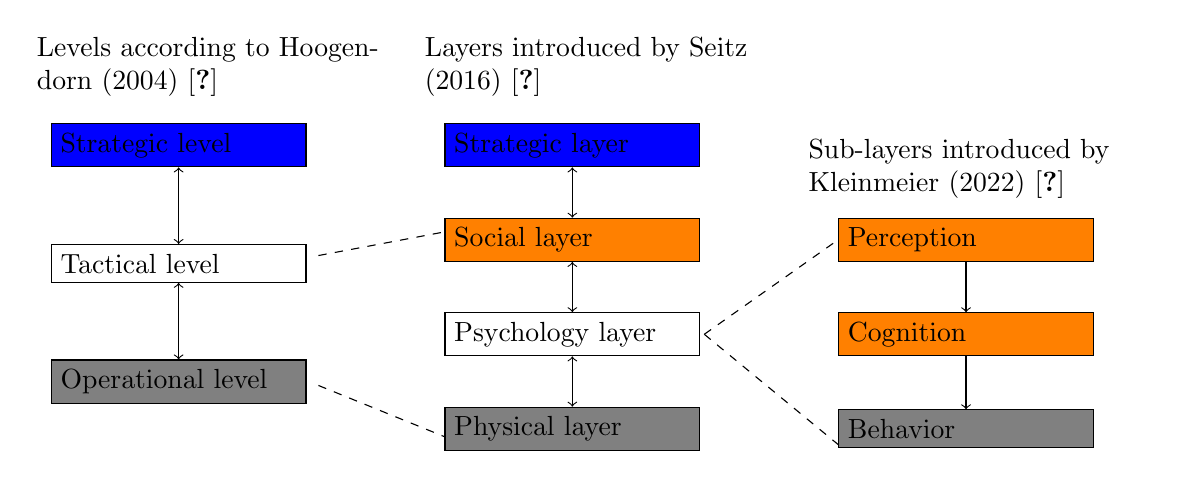
\begin{tikzpicture}[scale=1, transform shape]
\node[text width={4.5cm},anchor=west] at (-5.3, 1) {Levels according to Hoogendorn (2004)~\cite{hoogendoorn-2004-cdyn}};
 \node[fill=blue,anchor=west,rectangle,draw, text width=3cm] (strategie) at (-5,0) {Strategic level};
  \node[rectangle,draw,anchor=west,text width=3cm] (taktik) at (-5,-1.5) {Tactical level};
    \node[fill=gray,rectangle,draw,anchor=west,text width=3cm] (operational) at (-5,-3) {Operational level};
       \draw[<->](strategie) -- (taktik) ;
         \draw[<->](taktik) -- (operational) ;
         
            \draw[dashed] (-1.6,-1.4) -- (0,-1.1);
          \draw[dashed] (-1.6,-3.05) -- (0,-3.7);
                           
  \node[text width={4.5cm}] at (2, 1) {Layers introduced by Seitz (2016)~\cite{seitz-2016-cdyn} };
   \node[fill=blue,anchor=west,rectangle,draw,text width=3cm] (ip) at (0,0) {Strategic layer};
 \node[fill=orange,anchor=west,rectangle,draw,text width=3cm] (ic) at (0,-1.2) {Social layer};
  \node[rectangle,draw,anchor=west,text width=3cm] (b) at (0,-2.4) {Psychology layer};
    \node[fill=gray,rectangle,draw,anchor=west,text width=3cm] (bb) at (0,-3.6) {Physical layer};
 
 \draw[<->](ic) -- (ip) ;
         \draw[<->](ic) -- (b) ;
                  \draw[<->](b) -- (bb) ;

      
      \node[text width={4.5cm},anchor=west] at (4.5, -0.3) {Sub-layers introduced by Kleinmeier (2022)~\cite{kleinmeier-2021-cdyn} };
       \node[fill=orange,rectangle,draw,anchor=west,text width=3cm] (per) at (5,-1.2) {Perception}; 
 
      \node[fill=orange,rectangle,draw,anchor=west,text width=3cm] (cog) at (5,-2.4) {Cognition};
     \node[fill=gray,rectangle,draw,anchor=west,text width=3cm] (bah) at (5,-3.6) {Behavior};
     
              \draw[->](per) -- (cog) ;
                  \draw[->](cog) -- (bah) ;
     
     \draw[dashed] (3.3,-2.4) -- (5,-1.2);
          \draw[dashed] (3.3,-2.4) -- (5,-3.8);

        
\end{tikzpicture}
\caption[The hierarchical modeling approach for crowd behavior]{Hierarchical modeling approaches for crowd behavior. The hierarchic model approach introduced by Hoogendoorn~\cite{hoogendoorn-2004-cdyn} has been refined by Seitz~\cite{seitz-2016-cdyn} and Kleinmeier~\cite{kleinmeier-2021-cdyn}. The refinements allow to model collective, social and psychological behavior. }
\label{fig:hoogendoorn-hierarchisches-modell}
\end{figure}




\begin{figure}[hbt!]
\centering
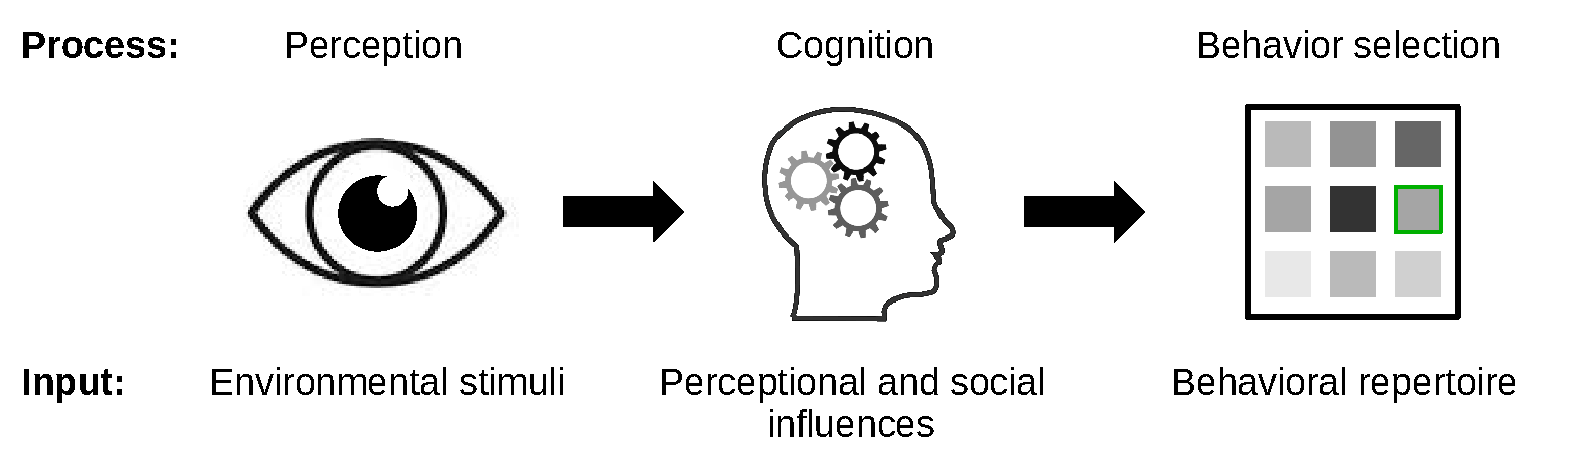
\includegraphics[width=1\textwidth]{../figures/state-of-the-art/crowds/perceptioncognigion.pdf} 
\caption[]{Modeling perception, cognition, and behavior selection.  At the perception layer, the most important stimulus is selected. At the cognition layer, a self-category is selected based on the most important stimulus and environmental conditions. From the self-category, a behavior is selected at the locomotion layer. Own graphics inspired by~\cite[p.89]{kleinmeier-2021-cdyn}.}
\label{fig:perceptioncognition}
\end{figure}




\FloatBarrier




\subsection{Modeling locomotion at the operational layer}

The movement behavior of a crowd is modeled at the operational level. The main inputs of a  locomotion model are a discretized topography with specified start and destination areas, and the crowd size. 

The granularity of the simulation output depends on the type of simulation model. Models can be divided into microscopic, mesoscopic, and macroscopic models~\cite{adrian-2019-cdyn}. Macroscopic models describe the flows of people as a continuum using macroscopic equations. This model group provides macroscopic output variables such as flows and densities. In a microscopic model, each pedestrian is modeled individually as so-called agent. Models from this category provide agent-specific output data, such as trajectories or individual waiting times. 
Mesoscopic models combine microscopic and macroscopic properties. Many of them are multiscale models~\cite{borrmann-2012-cdyn}:
Microscopic models are used in parts of the topography where detailed pedestrians locomotion is needed. Macroscopic models provide pedestrian flows in between these areas. 
Neither macroscopic nor mesoscopic models can capture psychological behavior in detail~\cite{kleinmeier-2021-cdyn}. In a crowd guidance system it is essential to model peoples' responses to route recommendations. Therefore, microscopic models are required. 

Several microscopic locomotion models have been developed in the last decades.
So-called \textit{cellular automatons}~\cite{gipps-1985-cdyn} are zero-order models that consider only the current state (`zero order of the derivative') in the propagation of the movement. The topography is discretized as a grid where each cell is either empty or occupied by a single agent. If a target cell is free and not a target of another agent, a move is executed. If multiple agents share the same target, the agent that has the higher probability is assigned to the cell. The so-called floor field modifies the probabilities to ensure that moves towards the target are preferred~\cite{kirik-2007-cdyn,schadschneider-2001-cdyn}.  

The \textit{Optimal Steps Model}~\cite{seitz-2012-cdyn} is a zero order model that is continuous in space and time. It was validated in several works~\cite{seitz-2016c-cdyn,seer-2015-cs,seitz-2012-cdyn,sivers-2016b-cdyn}. The basic idea is that agents try to improve a utility with every step~\cite{seitz-2012-cdyn}. The utility of each position in space is coded in a scalar function, also called floorfield. The utility, or potential, depends on the geodesic distance to the target and the proximity to other agents, see Fig.~\ref{fig:floorfield}. Utility increases when approaching targets and decreases when getting too close to obstacles and other agents. Physically spoken, agents, when moving, are attracted by targets and repulsed by obstacles and other agents. A dynamic floorfield can be used to model long- and medium-range interactions~\cite{koster-2014b-cdyn}. Sivers et al.~\cite{sivers-2015-cdyn} modified the potential functions based on Hall's theory of interpersonal distances. 





\begin{figure}[hbt!]
\centering
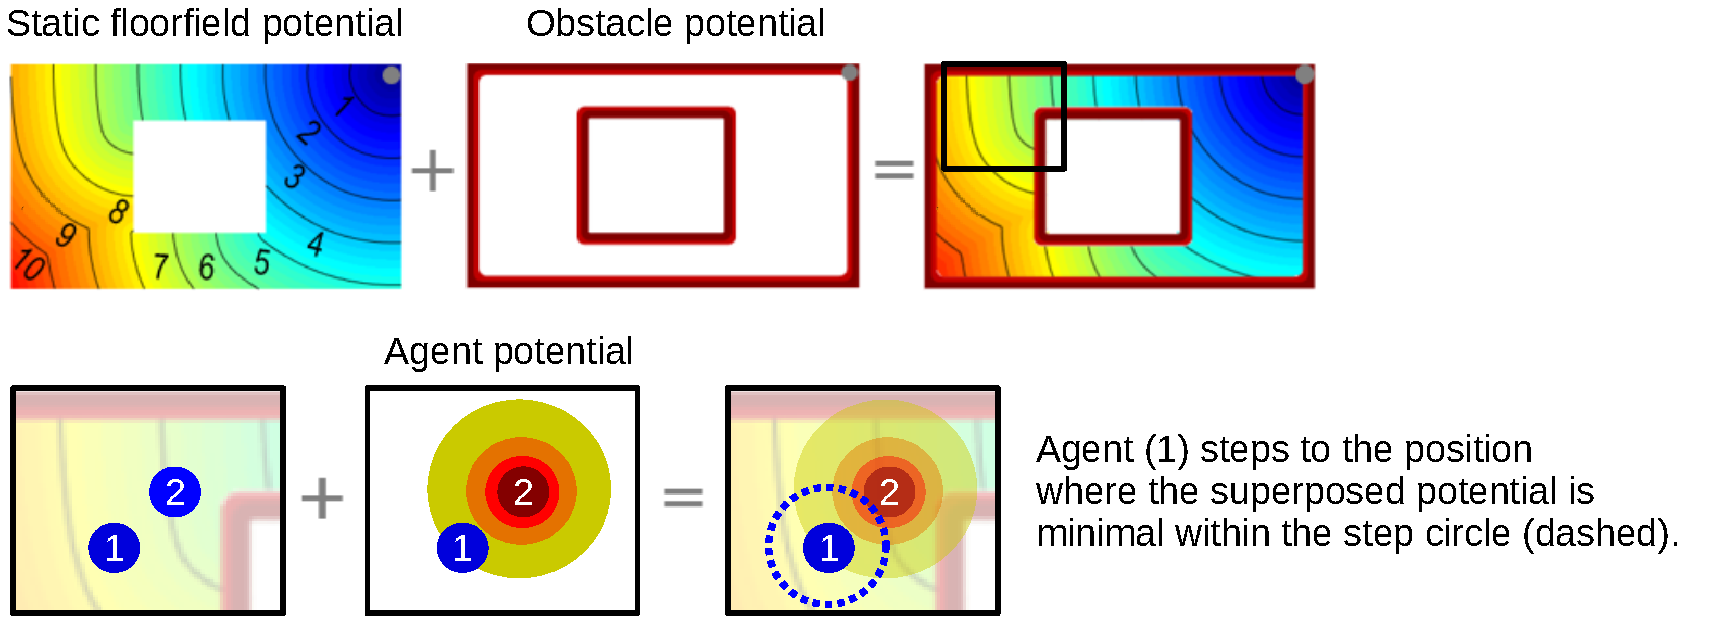
\includegraphics[width=1\textwidth]{../figures/state-of-the-art/crowds/optimalstepsmodel.pdf} 
\caption[Idea of the Optimal Steps Model]{Basic idea of the Optimal Steps Model~\cite{seitz-2012-cdyn}. Agents use the shortest path to a target (floorfield potential) while skirting obstacles (obstacle potential) and other agents (agent potential). The potentials are superposed. 
For each step, the optimal position needs to be found, that is, where the potential has a minumum within a step circle. }
\label{fig:floorfield}
\end{figure}



%
So-called \textit{Velocity-based Models} are first-order models that consider agents' position and speed (first derivative). In contrast to the cellular automaton, this model type is continuous in space.
Velocity-based models are either based on the concept of `optimal velocities' or the concept of `velocity obstacles'. In the `optimal velocities' approach, agents' velocity is adjusted using an optimal velocity function that depends on the minimum spacing in front~\cite{tordeux-2014-cdyn}. In the `velocity obstacles' approach, the orientation and the speeds are varied to find a configuration of agents where they do not collide~\cite{karamouzas-2009-cdyn}. 

So-called \textit{Force Models} are second-order models that employ accelerations (second spatial derivative) and force terms to model repulsion between agents and attraction to target. The most popular force model is the \textit{Social Force Model}~\cite{hirai-1975-cdyn,helbing-1995-cdyn} for which numerous extensions exist, see e.g.~\cite{chen-2018-cdyn}. Social Force Models are widely used in the pedestrian community despite numerical instabilities that can lead to oscillations~\cite{koster-2013-cdyn}.

Hybrid models combine the advantages of velocity-based and force-based models. This modeling approach includes the \textit{Gradient Navigation Model}~\cite{dietrich-2014-cdyn} where velocity and acceleration are considered in a decoupled manner: The position of the next step only depends on velocity-based quantities, but the magnitude of the velocity vector depends on an acceleration term.

So-called \textit{Decision-based or Decision Models} form another model category. These use simple rules for locomotion, such as `slow down', `keep a certain speed', or `accelerate' \cite{antonini-2006-cdyn}. One of them is the \textit{Behavioral Heuristics Model}~\cite{seitz-2016c-cdyn} that has four rules: (1) perform a step towards the target if the position is free. (2) If occupied try to evade tangentially. (3) If the tangential position is occupied perform a side step. (4) If the side is occupied wait.



Which locomotion model is most suitable for an applications depends how much computational effort one is willing to invest and on the required accuracy. Space-continuous models, such as force models or optimal steps models, produce more realistic trajectories than models with spatial discretization, such as the cellular automaton. However, such sophisticated models are computationally expensive: In the Optimal Steps Model an optimization problem needs to be solved for each step. The social force model requires solving a system of differential equations. If the scenario is large and low accuracy is acceptable, space discrete models, such as the cellular automaton, are still in use. Again, there is no model that fits all needs.












\subsection{Modeling route choice at the tactical layer}
Different types of models can be found at the tactical level: models for queuing behavior (see, e.g.,~\cite{kim-2013-cdyn}), models for avoiding crowds~(see, e.g.,~\cite{zoennchen-2013-cdyn}) , and small group models~(see, e.g.,~\cite{seitz-2011-cdyn}). 
Also route choice behavior is modeled at the tactical layer for which one can differentiate two model types, see~Fig.~\ref{fig:differencelinkchoiceroutechoice}.




Link choice models, or traffic assignment models, are used in traffic engineering to model the flow distribution at junctions~\cite{boyce-2021-cdynff}. They model the decision of the entire population depending on the current location in the traffic network. The input of such a model is the network topology and an origin-destination matrix. The output of the model is various route assignments for each origin-destination pair. The assignments are determined by optimizing the route assignments so that the average travel time~\cite{wardrop-1952-cdyn} or an alternative objective becomes minimum. 



\begin{figure}[hbt!]
\centering
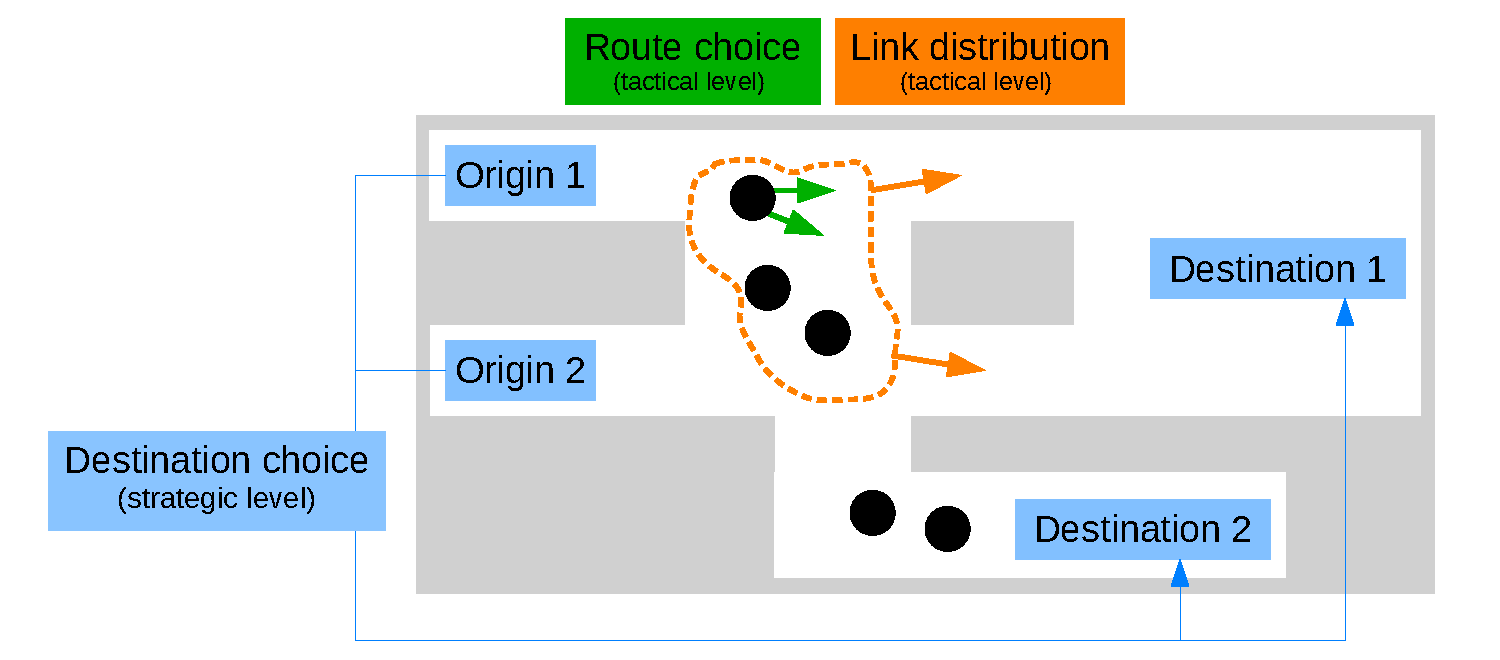
\includegraphics[width=11cm]{../figures/state-of-the-art/crowds/abgrenzung.pdf} 
\caption[Zusammenhang zwischen Modellen des strategischen und taktischen Layers]{Relationship between strategic and tactical layer models.
Route choice models capture individual route choice, while link choice models simulate the route distribution of a population. So-called destination~\cite{danalet-2015-cdyn} and location choice models~\cite{beaulieu-2019-cdyn} belong to the strategic layer.
}
\label{fig:differencelinkchoiceroutechoice}
\end{figure}

Route choice models reflect the decision-making process of an individual. Therefore, they belong to the cognition layer of Kleinmeier's psychology layer~\cite{kleinmeier-2021-cdyn}.
Numerous experiments have been conducted to identify factors or stimuli that affect the route choice, see e.g. \cite{palma-2012-cdyn,crociani-2016b-cdyn,kinateder-2018-cdyn}. 
Many route choice models are multi-logit models that make a route decision based on environmental and exogenous factors~\cite{lopez-2021-cdyn}. 
Shi et al.~\cite{shi-2023-cdyn} propose a conditional multinomial logit model to model the route choice behavior of metro passengers. Daamen~\cite{daamen-2004-cdyn} proposes a logit model that models route choice with the factors of walking and waiting times, route lengths, and walking comfort.
Xu et al.~\cite{xu-2014-cdyn} suggest a model that considers the distance to the exits and their attractiveness. 
Ramos et al.~\cite{ramos-2020-cdyn} use the travel time as a factor in their logit model. 
Tong et al.~\cite{tong-2021-cdyn} extend a logit model proposed by Arganda et al.~\cite{arganda-2012-cdyn} by adding a factor that has the effect that people become "less sensitive to environmental information the more decisions they have to make". In a second study, Tong et al.~\cite{tong-2021b-cdyn} propose to add another factor that models the so-called ‘route commitment effect’, that is,  "the more pedestrians invest into a planned route by walking along it, the more likely they are to adhere to this route even when encountering congestion". 
Other logit models consider stairs~\cite{aleksandrov-2018-cdyn}, visibility conditions~\cite{lovreglio-2016-cdyn,haghani-2018b-cdyn}, the tendency to stick to a route~\cite{haghani-2019c-cdyn}, or the effect of instructions from human guides~\cite{nishida-2023-cdyn}. Apart from route choice models, machine learning has been  proposed to emulate route choice behavior, see e.g.~\cite{zhao-2023-cdyn}.


Few approaches try to model people's compliance to instructions:
Lopez~\cite{lopez-2021-cdyn} split agents into two groups. For non-compliant agents, they use a route choice model. Compliant agents follow the instruction, ignoring other factors.
Haghani et al.~\cite{haghani-2019c-cdyn} use another approach: They implicitly model compliance by introducing a factor called ‘inertia’ to a logit model that biases the decision.




As one can see there are several suggestions to model route choice behavior. All of the proposed models were derived for different factors and scenarios. 
Consequently, the models cannot be simply transferred to arbitrary scenarios. Moreover, there is no approach that models the compliance with route recommendations provided by a mobile application. Therefore, a new modeling approach is needed.




\subsection{Modeling of communication and psychological factors}
How people respond to information depends on how information is communicated, see e.g.~\cite{carter-2015-life}. There are different approaches to model communication aspects. 
Templeton et al.~\cite{templeton-2023-cdyn} distinguishes four principle modeling strategies:

\begin{itemize}
\item Field of influence: Agents have a bounded field of influence around them, which transmits information to other agents. See e.g. \cite{bernardini-2014-cdyn}.
\item Network-based: Agents share information with others within their social network. See e.g. \cite{yang-2019-cdyn}.
\item Information trails: Agents disseminate information via trails in the environment as they move. See e.g.~\cite{zheng-2019-cdyn}.
\item External information: Agents in particular areas become informed by an external source. See e.g. \cite{rigos-2019-cdyn}.
\end{itemize} 

Some other approaches aim to model the effect of the emotional state of an individual. Pelechano et al.~\cite{pelechano-2005-life} propose a model in which the decision-making process depends on the emotional state affected by stress and physiological factors. Bosse et al.~\cite{bosse-2013-life} model the effect of beliefs, desires, and intentions. Kielar~\cite{kielar-2017-cdyn} takes  memory and individual preferences into account. %Pan~\cite{pan-2006-cdyn} 
Wijermans~\cite{wijermans-2011-cdyn} considers the effect of the physiological constitution.
 
Some approaches focus on modeling social identities (Section~\ref{sec:crowdbah}). In her dissertation, Sivers~\cite{sivers-2016c-cdyn} modeled the effect of social identities on helping behavior. Kleinmeier~\cite{kleinmeier-2021-cdyn} investigated how cooperative behavior between group members can be modeled using self-categories.

The brief overview shows that there are indeed approaches for modeling psychological changes and the communication in a crowd. However, it is unclear how one can model the effect of route recommendations that are communicated via mobile applications in combination with social identities in a crowd guidance system. 




\subsection{Simulation frameworks}
\label{sec:crowdssimframeworks}

Several open-source simulation frameworks are available to simulate crowd behavior, see Tab.~\ref{tab:overviewcrowdsimulators}. Some of them are no longer maintained. Most of them operate at the operational layer, that is, providing locomotion simulation. The only simulator providing a psychology layer is the \textit{Vadere} simulation framework~\cite{kleinmeier-2021-cdyn}.



\begin{table}[hbt!]
\begin{footnotesize}

\begin{tabular}{p{2.7cm}p{3.3cm}p{2.5cm}p{1.8cm}p{1.8cm}}
\hline
\textbf{License} & \textbf{ Simulator} & \textbf{Language} & Reference & Maintained \\
\hline
LGPL & JuPedSim & C++,Python  &\cite{chraibi-2016-cs}\\
LGPL & Vadere & Java & \cite{kleinmeier-2019-cdyn}\\
GPLv3 & GAMA & Java & \cite{taillandier-2017-cdyn}\\
MIT & Agents.jl & Julia & \cite{datseris-2022-cdyn}\\
LGPL v3 & jCrowdSimulator & Java & \cite{meinert-2019-cdyn}  \\
GNU GPL & Cromosim &  Python & \cite{maury-2019-cdyn}  \\
Apache 2.0  & Mesa & Python & \cite{masad-2015-cdyn}\\
\hline
GPLv3 & PedSim & JavaScript & \cite{gloor-2005-cdyn}  & no \\
Apache 2.0 &  Menge & C++ & \cite{curtis-2016-cdyn} & no \\
- & FDS+Evac  & Fortran & \cite{korhonen-2007-cdyn} & no \\
- & MomenTUMv2 & Java & \cite{kielar-2016b-cdyn} &  no \\
 \hline
%Commercial & AnyLogic & Java  \\
%& crowd:it & Java\\
%& PD Pedestrian Dynamics & 4DScript \\
%& MassMotion  & Python,Java,C++,C\# \\
%& Crowd.lab & C++,JavaScript \\
%& SimWalk & C++ \\
%& PTV Vissim & Unknown \\
%& UCrowds & C++ &  \\

\end{tabular}
\end{footnotesize}
\caption[]{Overview on open-source software for crowd simulations. The list is based on Richard's software review~\cite{richards-2020-cdyn}. I consider simulators as no longer maintained when the last commit was before Dec 2022 (checked: 18 Jan 2024). }
\label{tab:overviewcrowdsimulators}
\end{table}


\section{Modeling mobile networks and direct communication}

\label{sec:modelcom}


This section belongs, like the previous section, to the second part of the state of the art. I present the state-of-the-art of modeling and simulating direct communication in mobile networks. First, standards on mobile communication and their respective protocol stacks are introduced. Then, an overview of channel modeling is given. Finally, I present state-of-the-art system level simulators. I assume that the reader is familiar with the ISO/OSI reference model and the basic principles of radio wave propagation such as \enquote{free-space (or line-of-sight) propagation, transmission (and absorption), specular reflection, diffraction, and diffusion (also known as diffuse scattering) [...]}~\cite{rappaport-2001-com}. If not, I recommend to~\cite{rappaport-2001-com}.



\subsection{Overview of mobile standards enabling direct communication}

For enabling device-to-device (D2D) communication, two main technologies have emerged: dedicated short-range communication based on the IEEE 802.11p standard~\cite{802.11p-2010-com} and cellular vehicle-to-everything (C-V2X) communication based on several releases of the 3rd Generation Partnership Project (3GPP), see Fig.~\ref{fig:protocollstack}.
% .There are also approaches to enable direct communication via 5G mmWave.


\begin{figure}[hbt!]
\centering
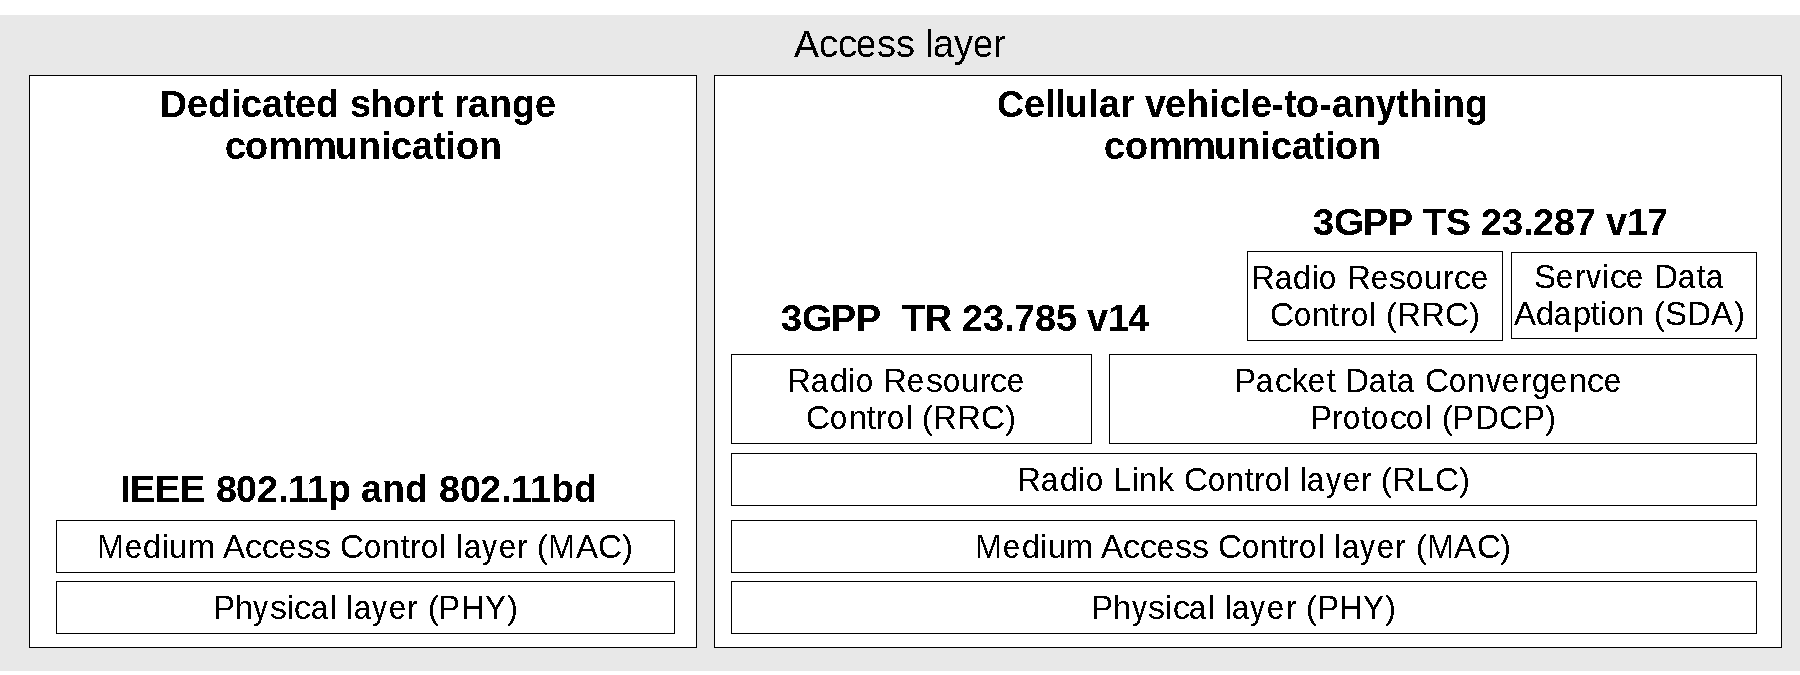
\includegraphics[width=\textwidth]{../figures/state-of-the-art/mobilecommunication/protocollstacks.pdf} 
\caption{Protocol stack reference model for direct communication. Standards for direct communication specify the lower layers of the protocol stack.  Own graphics, inspired by~\cite[p.89]{chen-2023-com}. }
\label{fig:protocollstack}
\end{figure}



\subsubsection{Dedicated Short Range Communication}

The \textit{IEEE 802.11p} standard~\cite{802.11p-2010-com} was the first mobile standard enabling Device-to-Device~(D2D) communication. It specifies Dedicated Short Range Communication (DSRC) on the physical layer and on the medium access control (MAC) layer. At the physical layer, the Orthogonal Frequency Division Multiplexing (OFDM) is specified for the modulating of data on multiple carrier frequencies.
At the medium access control (MAC) layer, the standard specifies the Enhanced Distributed Channel Access (EDCA) method that employs carrier sense multiple access with collision avoidance (CSMA/CA): Before a packet is sent, the network node checks whether the transmission channel is free. If the channel is busy, the node waits for a randomly defined period of time and then checks again.
Therefore, participants access the channel in a self-organized, decentralized way. However, this requires that devices recognize the channel occupation correctly and do not start accessing the channel simultaneously. Therefore, the performance depends on the density of participants. The more participants, the more likely are collisions and interference that lead to packet loss~\cite{shrestha-2020-com}. It cannot be guaranteed that packets arrive within a certain time~\cite{shrestha-2020-com}.

As the 802.11p standard only applies to the physical and medium access control layer, the standard is combined with other standards to enable Dedicated Short Range Communication. In the context of Intelligent Traffic Systems (ITS), there are the IEEE 1609 standard~\cite{ieee-2016-IEEEStd1609.4-com} (USA), the CEN/ETSI EN302 663 standard~\cite{etsi-2019-EN302663-com} (Europe) and the ARIB STD-T109 standard~\cite{its-2012-T109-com} (Japan). An overview of the country-specific specifications can be found in~\cite{costandoiu-2019-com}.
The transmission is intended to operate in the frequency range 5855\,MHz to 5925\,MHz. 

The \textit{IEEE 802.11bd} standard~\cite{ieee802.11bd-2022-com} is an amendment of the set of 802.11 standards. It was released in 2023, and it is interoperable with the 802.11p technology. The amendment aims to improve throughput, latency, reliability, and range through new specifications for the physical layer and the medium access layer~\cite{yacheur-2020-com}.  Therefore, 802.11bd-based technology is more advanced than \textit{IEEE 802.11p} technology. The bandwidth of the channel is $20\,MHz$ which is twice the bandwidth of the IEEE 802.11p standard. Like the IEEE 802.11p, the amendment specifies the EDCA method for accessing the channel. Due to the larger bandwidth and adjustments regarding the error correction scheme, more packets can be transmitted~\cite{yacheur-2020-com}. 
Although the 802.11bd amendment has improved network performance compared to the 802.11p standard, 802.11bd-based technology can often not outperform Cellular Vehicle-to-everything communication, as demonstrated in~\cite{anwar-2019-com}.


\subsubsection{Cellular Vehicle-to-everything communication}
Cellular Vehicle-to-everything communication (C-V2X) has been developed by the Third Generation Partnership Project (3GPP), see Fig.~\ref{fig:overviewofreleases3gpp}. 


\begin{figure}[hbt!]
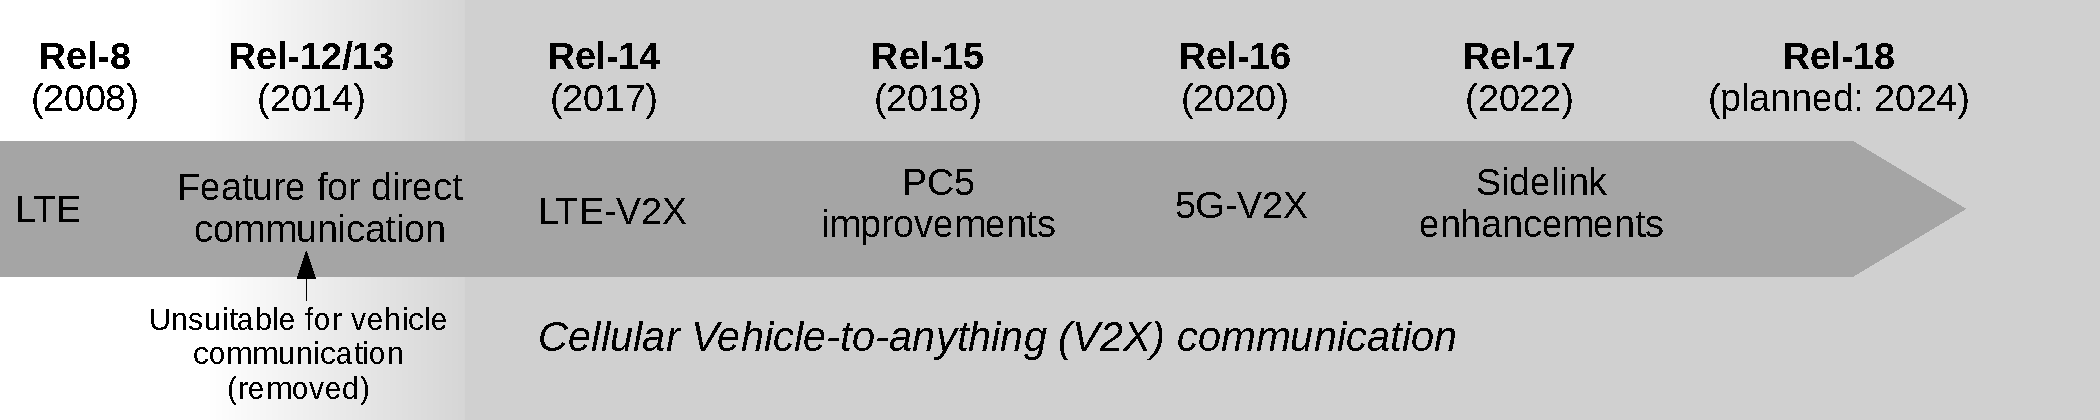
\includegraphics[width=\textwidth]{../figures/state-of-the-art/mobilecommunication/release3gpp.pdf} 
\caption{Standards of the 3rd Generation Partnership Project (3GPP) for Cellular Vehicle-to-everything communication. Own graphics; inspired by~\cite{bazzi-2021-com}.}
\label{fig:overviewofreleases3gpp}
\end{figure}


\textit{LTE V2X}, that is Vehicle-to-everything communication over Long Term Evolution networks, is specified in the technical reports TR 22.885~\cite{3gpp-22.885-2015-com} and TR 36.885~\cite{3gpp-36.885-2016-com} as well as in the technical specifications TS 22.185~\cite{3gpp-22.185-2020-com}, TS 23.285~\cite{3gpp-23.285-2020-com}, TS 36.213~\cite{3gpp-36.213-2020-com}, TS 36.321~\cite{3gpp-36.321-2020-com} released by the 3GPP. Direct communication is specified over the PC5 interface using so-called sidelinks. The sidelink uses the same band for communication as the Dedicated Short Range Communication: $5.9\,\text{GHz}$.
Two communication modes exist: the controlled mode (mode 3) and the autonomous mode (mode 4), see Fig.~\ref{fig:scenariosmodes}. In mode 3, a base station allocates resources. In this mode it is not specified whether dynamic or semi-persistent scheduling is employed~\cite{bazzi-2021-com}. 
For the autonomous mode a semi-persistent scheduling procedure is required: each network participant allocates frames and sub-channels at a fixed time interval based on channel occupancy estimates~\cite{bazzi-2021-com}. 



\begin{figure}[hbt!]
\centering
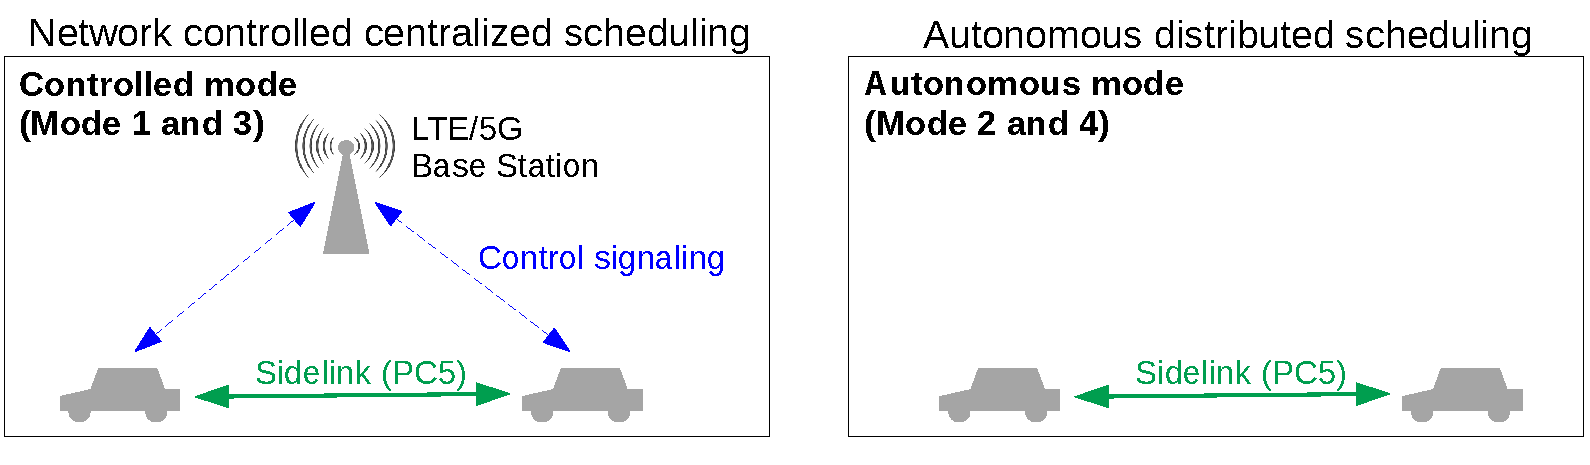
\includegraphics[width=1.0\textwidth]{../figures/state-of-the-art/mobilecommunication/cellularmodes.pdf} 
\caption[Direct communication scenarios in a cellular network]{Modes for cellular vehicle-to-everything communication. Vehicles (or devices) share data directly over the PC5 interface using so-called sidelinks. In mode 1 (5G) and 3 (LTE) the base station allocates resources to reduce the risk of  collision and interference (left). In mode 2 (5G) and 4 (LTE), vehicles schedule packet transmissions autonomously~\cite{bazzi-2021-com}.  }
\label{fig:scenariosmodes}
\end{figure}





\textit{5G V2X} or \textit{NR-V2X}, where NR stands for `New Radio', means communication over sidelinks in networks of the fifth generation (5G). The 5G sidelink is defined by the 3GPP in the documents TR 22.886~\cite{3gpp-22.886-2018-com}, TR 38.885~\cite{3gpp-38.885-2019-com}, TS 23.287~\cite{3gpp-23.287-2020-com}, TS 22.186~\cite{3gpp-22.186-2019-com}, TS 38.213~\cite{3gpp-38.213-2020-com}, TS 38.321~\cite{3gpp-38.321-2020-com} and TS 37.895~\cite{3gpp-37.895-2020-com}. 
5G sidelinks and LTE sidelinks differ in their waveform, the scheduling interval, and the channel coding procedure, see Tab.~\ref{tab:directcom-overview}. As with LTE sidelink communication, one can distinguish a controlled (mode 1) and autonomous mode (mode 2). 
Importantly, the 5G sidelink operates at two frequency bands: $0.41\,\text{GHz}$-$ 7.125\,\text{GHz}$ and $24.25\,\text{GHz}$-$52.6\,\text{GHz}$. For the latter, the wavelength is at the scale of a millimeter, which is why it is referred to as 5G millimeter waves (mmWaves). 






\subsubsection{Overview on technologies and interoperability}
An overview of specifications and technologies can be found in Tab.~\ref{tab:directcom-overview}.
Importantly, dedicated short range communication technologies and cellular technologies are not interoperable~\cite{molina-2020-com}. Even in a `hybrid system', the technologies operate simultaneously but independently~\cite{shrestha-2020-com}.
The 802.11bd standard~\cite{ieee802.11bd-2022-com} is compatible with its predecessor IEEE 802.11p. The LTE sidelink and the NR sidelink are basically not interoperable, but they can co-exist~\cite{bazzi-2021-com}. 



\begin{table}[hbt!]
\begin{footnotesize}
\begin{tabular}{|p{2.4cm}|p{2.5cm}|p{2.5cm}|p{2.5cm}|p{2.5cm}|}
\hline 
\textbf{Standard} & \textbf{802.11p} &  \textbf{802.11bd} & \textbf{LTE V2X} & \textbf{5G/NR V2X} \\ 
\hline 
Technology & WLAN & WLAN & 4G/LTE & 5G \\ 
\hline 
First release & 2012 & 2023 & 2017/18 (3GPP Rel-14/15) & 2020 (3GPP Rel-16)  \\ \hline
Wave form & OFDM & OFDM & SC-FDMA & OFDM \\ 
\hline 
Ressource allocation & decentral & decentral  & central (Sidelink mode 3), decentral (Sidelink mode 4) &  central (Sidelink mode 1), decentral (Sidelink mode 2) \\ \hline

Modes & Broadcast & Broadcast, groupcast & Broadcast & Broadcast,
groupcast, unicast
\\ \hline 
Range & short range &  short range & extended range
 & extended range \\ 
\hline 
Scheduling interval &None& None & One sub-frame & Slot, mini-slot or multi-slot \\
\hline
Channel coding & Binary Convolutional Coding (BCC)  & LDPC & Data: Turbo, 
Control: Convolution & Data: LDPC, Control: Polar 
\\ \hline 
Frequency band & 5.9\,GHz & 5.9\,GHz/ 60\,GHz & 5.9\,GHz &  0.41\,GHz-7.125\,GHz, 24.25\,GHz-52.6\,GHz (mmWave) \\ \hline 
Sub-carrier spacing &  156.25\,KHz & 312.5\,KHz, 156.25\,KHz, 78.15\,KHz & 15\,KHz & 15\,KHz, 30\,\,KHz, 60\,KHz, 120\,KHz \\ \hline 
Retransmission & None  & Congestion dependent & Blind & HARQ-based \\ 
%Cyclic Prefix (CP) & 1.6 us & 1.6 us and 3.2 us  & & \\
%High density support & Packet loss at high density & • & No packet loss guaranteed
%at high density & • \\ 
%Security and Privacy
% & Yes (based on IEEE WAVE \&
%ETSI ITS security services) & Yes (based on IEEE WAVE \&
%ETSI ITS security services) & Yes (based on IEEE WAVE \&
%ETSI ITS security services) & Yes (based on IEEE WAVE \&
%ETSI ITS security services) \\  
%\hline 
%Latency & Low  V2V
%communications & • & Round trip latency less than 1ms & • \\ \hline 
\hline 
\end{tabular} 
\end{footnotesize}
\caption[Overview of standards for direct communication]{Overview of standards for direct communication. The IEEE technologies are not interoperable with cellular technologies. The table is based on the data from~\cite{shrestha-2020-com,bazzi-2021-com,molina-2020-com}.}
\label{tab:directcom-overview}
\end{table}














\subsection{Modeling wireless propagation channels}
For a mobile network simulation, it is essential to model the propagation channel.
\enquote{A wireless propagation channel is the medium linking the transmitter and the receiver. Its properties determine the information-theoretic capacity, i.e., the ultimate performance limit of wireless communications, and also determine how specific wireless systems behave. It is thus essential that we know and understand the wireless propagation channel and apply this knowledge to system design.}~\cite[p.45]{molisch-2011-com}. 

\newpage

Molisch~\cite[p.125ff]{molisch-2011-com} distinguishes three basic modeling approaches:
\begin{itemize}
\item `Deterministic' channel modeling: solve Maxwell's equation to compute channel characteristics. Since solving the integrals or differential equations is time-consuming, ray-based methods are used in practice. This approach is often applied in network planning and system deployment.
\item `Stochastic' channel modeling: use models to estimate statistical properties of the channel characteristics. This approach is often applied when designing and comparing systems.
\item Use of measurement data: use empirical data to describe the channel characteristics. The execution of a model is not necessary. This approach is often applied when measurement data is available for a specific scenario.
\end{itemize}

Channel models can be classified according to their temporal and spatial resolution~\cite[p.70]{rappaport-2001-com}: so-called large-scale propagation models predict the average signal strength over the distance and are typically used to estimate the coverage. Small-scale or fading models model the signal strength at a fine local (wavelengths) and temporal (seconds) scale~\cite[p.70]{rappaport-2001-com}.


Four channel model categories are differentiated~\cite{molisch-2011-com}, see Fig.~\ref{fig:pathlossmodelsoverview}. Narrowband models describe the signal attenuation. Wideband models focus on the dispersion of the signal. Directional models capture directional properties of signal components, which is why these models are suitable for the simulation of multi-antenna systems~\cite[p.445]{molisch-2011-com}. `Deterministic' models are based on Maxwell's theory of wave propagation.

\begin{figure}[hbt!]
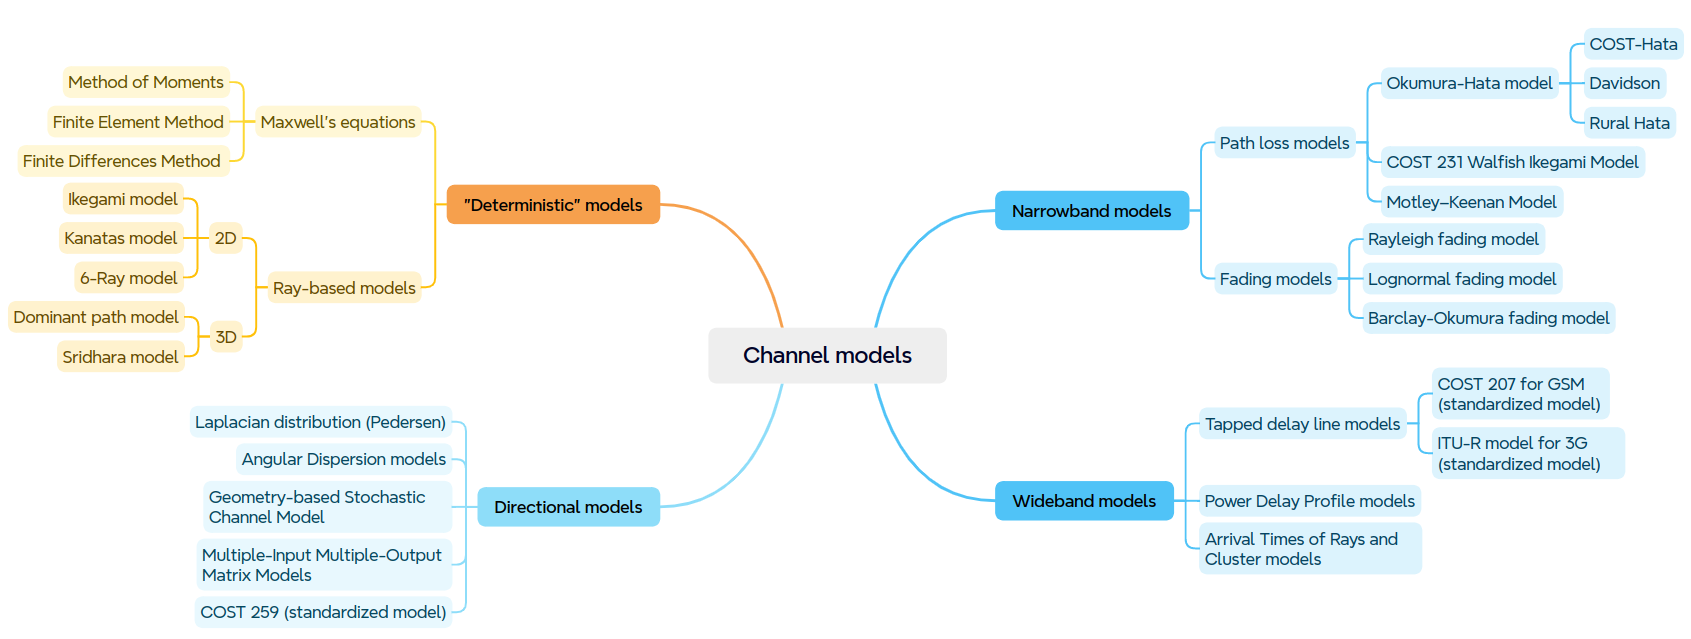
\includegraphics[width=1.0\textwidth]{../figures/state-of-the-art/mobilecommunication/channelmodelv2.png} 
\caption{Classification of channel models according to Molisch~\cite{molisch-2011-com}. The model examples come from Molisch~\cite{molisch-2011-com} and Phillips et al.\cite{phillips-2013-com}. Own graphic inspired by \cite{molisch-2011-com,phillips-2013-com}.}
\label{fig:pathlossmodelsoverview}
\end{figure}

Apart from that, there are different approaches how a channel can be represented as model. Phillips et al.~\cite{phillips-2013-com} distinguishes several categories: (1) Theoretical models are derived analytically from the theory of ideal electromagnetic propagation. An example is the free space path loss model according to Friis~\cite{friis-1946-com} that describes how the power decreases quadratically over the distance between transmitter and receiver. An extension of Friis' model is the Two-Ray Ground Reflection model that considers reflections from the ground~\cite[p.95]{rappaport-2001-com}. 
%
The second category is formed by so-called (2) basic models that are derived from empirical data. 
The Okumura-Hata Model~\cite{okumura-1968-com} describes the path loss depending on the distance between sender and receiver, the frequency, and the height of the base station or mobile station. The model is intended for scenarios with an elevated station, e.g., at a rooftop. Numerous extensions exist, such as the COST Hata Model, which is applicable even for frequencies above $1500\,$MHz~\cite{hata-2023-com}. 


For outdoor scenarios so-called (3) terrain models are used. They are similar to basic models but also consider diffraction. Stochastic fading models (4) add a random variable to capture fading. Models from this category are typically used to design the physical or link layer~\cite{phillips-2013-com}. One of them is the Lognormal Shadowing Model, which can be considered a stochastic version of Friis model with a variable decay parameter. Stochastic fading models, such as the Rayleigh Fading model~\cite{sklar-1997-com}, model small-scale effects. 
Ray-based models (5)  try to capture the effect of wave propagation in the entire space using rays. Supplementary models (6) adjust the results of other models. Many of these models focus on adjusting the signal propagation due to obstacles such as trees or walls, see e.g.~\cite{durgin-1998-com,jong-2004-com,torrico-1998-com}. The so-called ideal obstacle loss model~\cite[p.75]{virdis-2019-com} models the extreme case: If an obstacle is in the line-of-sight, the signal strength is zero. More model examples can be found in~\cite{phillips-2013-com}. 



%\subsection{Overview of standardized channel models}
Standardized channel models are established models that are used by the mobile networks community to develop higher layer protocols and applications.
They are released by standardization institutions such as 3rd Generation Partnership Project  or IEEE, see Tab.~\ref{tab:standardchannelmodels}. The models have been extensively calibrated or validated using empirical data and simulation data, see \cite{erceg-2004-com, winner-2007-com,3gpp2-2003-com,3gpptr36873-2017-com,liu-2012-com,itu-2017-com,tr38901-2018-com,raschkowski-2015-com,peter-2017-com,jaeckel-2019-com} and their references.  I do not want to develop direct communication technologies further, but I want to test their suitability for crowd management applications. Therefore, I employ standardized models for my investigations.
 

\begin{table}[hbt!]
\begin{footnotesize}
\begin{tabular}{p{2.0cm}p{1.2cm}p{6.5cm}p{3.2cm}}
\hline 
{Standard} & {Year} & {Channel model} & {Gremium} \\
\hline
802.11n & 2004 & 802.11n channel model \cite{erceg-2004-com} & IEEE \\
%802.15.3a/4a & 2003/4 & 802.15.3a/4a channel model \cite{molisch-2003-com,molisch-2004-com} & IEEE \\
%802.16 & 2001 & SUI model \cite{erceg-2001-com} & IEEE \\
LTE & 2007 & WINNER model \cite{winner-2007-com} & WINNER project \\
LTE & 2003 & 3D Spatial Channel Model (TR 25.996) \cite{3gpp2-2003-com} & 3GPP \\
LTE & 2017 & 3D Channel Model (TR 36.873) \cite{3gpptr36873-2017-com} & 3GPP \\
LTE & 2012 & COST 2100 model \cite{liu-2012-com} & COST 2100 \\
5G & 2017 & ITU-R channel model \cite{itu-2017-com} & ITU-R \\
5G & 2018 & 3GPP TR 38.901 \cite{tr38901-2018-com} & 3GPP \\
5G & 2015 & METIS \cite{raschkowski-2015-com} & European Commission \\
5G & 2017 & mmMAGIC \cite{peter-2017-com} & Frauenhofer \\
5G & 2019 & QuaDRiGa \cite{jaeckel-2019-com} & Frauenhofer \\
\hline 
\end{tabular} 
\end{footnotesize}
\caption{Examples of standardized channel models. Several models are available for modeling radio channels for different network technologies.  These models are typically used for the development of protocols and applications at higher layers, such as the application layer. }
\label{tab:standardchannelmodels}
\end{table}



\subsection{Simulation frameworks}
\label{sec:mobilenetworkssimulationframeworks}

System-level simulators provide, in contrast to link-level simulators, implementations of the full protocol stack. An overview of simulators can be found in Tab.~\ref{tab:overviewcrowdsimulators}.
Only the two simulation frameworks \textit{OMNeT++}~\cite{varga-2019-com} and \textit{ns-3}~\cite{riley-2010-com} have established themselves as scientific open-source software. The frameworks and their related model libraries provide implementations for standardized channel models including the channel. For example, the 3D channel model TR 36.873~\cite{3gpptr36873-2017-com} is available in the \textit{simu5G}~\cite{3gpptr36873-2017-com} simulator that belongs to the \textit{OMNeT++} ecosystem~\cite{nardini-2020b-com}.


\begin{table}[hbt!]
\begin{tabular}{p{2.7cm}p{3.2cm}p{2.5cm}p{1.8cm}p{1.8cm}}
\hline
{Simulator} & {License} & {Language} & Reference & Maintained \\
\hline
OMNeT++ & Academic public & C++ & \cite{varga-2019-com} \\
ns-3 & GNU GPLv2 & C++, Python & \cite{riley-2010-com} \\ 
GloMoSiM & Academic public & Parsec, Java & \cite{zeng-1998-com} & no \\
LTE-SIM & GPL-3.0 license & C, C++& \cite{piro-2011-com} & no\\
Jist/Swans & CRF & Java & \cite{barr-2004-com} & no\\ \hline
\end{tabular}
\caption[]{Overview of open source software for mobile network simulations. The list is based on Khan's software review~\cite{khan-2012-com}. I consider simulators as no longer maintained when the last commit was before Dec 2022 (checked on 25 Jan 2024). }
\label{tab:overviewcrowdsimulators}
\end{table}

Different studies demonstrate that the mobility behavior of mobile nodes has a major impact on the  mobile network simulation: Wischhof et al.~\cite{wischhof-2022b-com} demonstrated that the results of the mobile networks simulation depend on the accuracy of the locomotion model.
Bai et al.~\cite{bai-2004-com}  found  that path duration in ad hoc networks depends on the accuracy of node movement. They tested different mobility models. Chancay-Garc\'{i}a et al.~\cite{chancay-2018-com} found that information dissemination depends on the degree of motion and message size. 
For this reason, \textit{OMNeT++} and \textit{ns-3} have an interface that allows one to use pre-generated mobility traces in the network simulation. It is also possible to obtain position data online from the SUMO simulator over an interface~\cite{wegener-2008-com}. 

The SUMO simulator~\cite{wegener-2008-com} provides simple pedestrian models where agents move, for example, along lanes like vehicles. These models are not validated against empirical data from pedestrian dynamics research. It cannot be ensured that they produce realistic trajectories. Consequently, safety-critical pedestrian densities cannot be evaluated reliably. I conclude that it is essential to use a validated locomotion model in the investigation of a crowd guidance system. Because several crowd models and simulators are already available (Section~\ref{sec:crowdssimframeworks}), I look at model and simulator coupling in the next section.


%Therefore it is necessary to use validated pedestrian mobility models when investigating the suitability of a mobile communication for the redirection of crowds. 

\FloatBarrier


\section{Model composition and coupling}
\label{sec:simulationframeworks}

In the previous sections (Sections~\ref{sec:modelcrowd}-\ref{sec:modelcom}), I introduced crowd models and mobile network models. These models are separate models that are usually executed independently from each other. For the simulative investigation of a crowd guidance system, these models need to be connected. In this section, I present state-of-the-art approaches how separate models and simulators can be coupled. First, model coupling is discussed for different system types. Next, sequential update procedures are introduced. Then, it is discussed how the data exchange between simulators can be realized. Finally, state-of-the-art simulation frameworks and interfaces are presented.

\subsection{Coupling models and simulators}
With model coupling, two different component models are connected so that they can exchange information with each other.  What a model coupling looks like depends strongly on the structure of the system, see Fig.~\ref{fig:modelcouplingapproaches}. In partitioned multi-physics systems, the model coupling is located at a geometric boundary. Both components share a system state at the boundary. To couple models, the \textit{monolythic approach} or the \textit{partioned approach} can be used. 
\enquote{The monolithic approach, on one hand, uses a single system of equations to describe and solve the coupled problem. On the other hand, partitioned methods use existing single-physics solvers and couple them to a simulation that strives to solve the overall coupled problem}~\cite[p.16]{lindner-2019-cs}.  


\begin{figure}[hbt!]
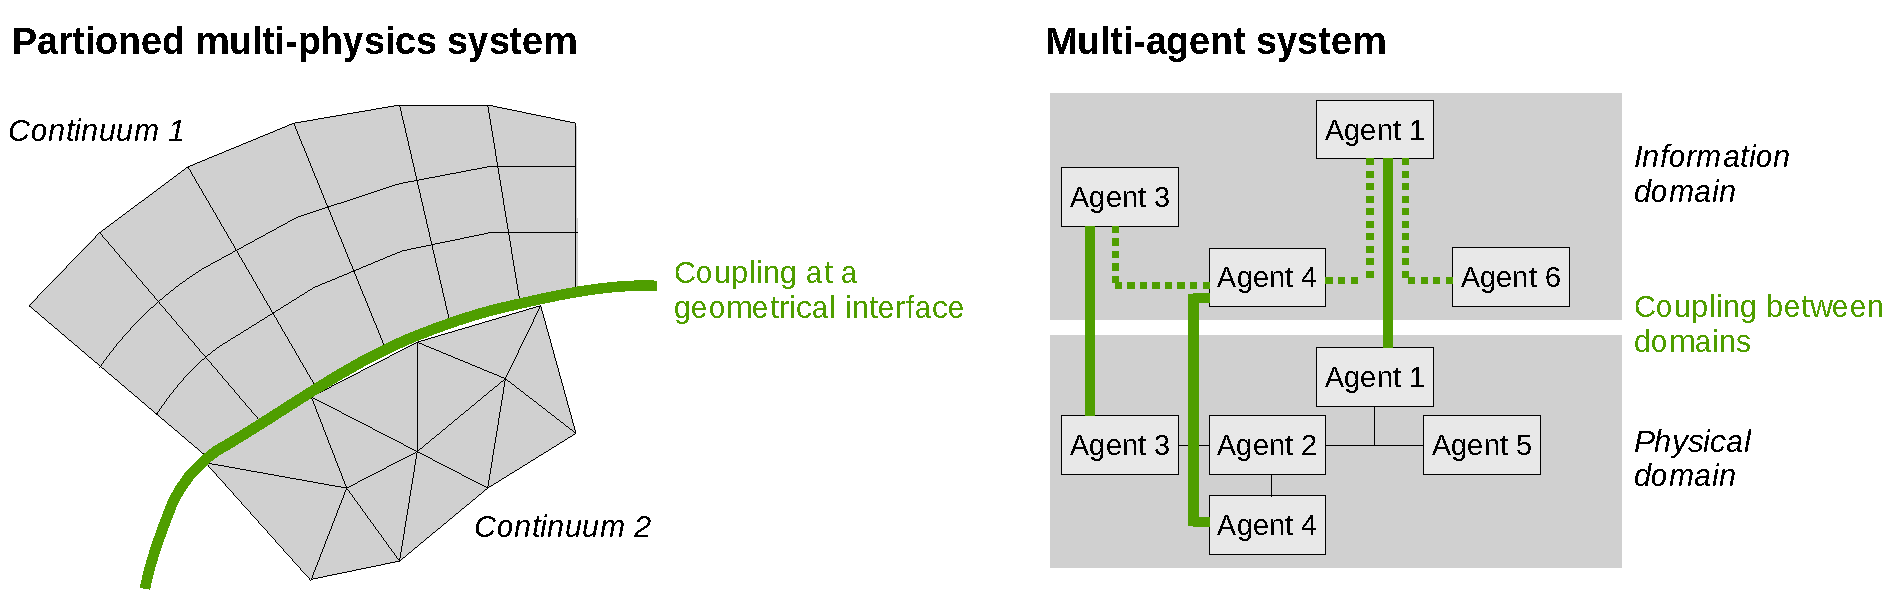
\includegraphics[width=\textwidth]{../figures/state-of-the-art/coupling/modelcouplingapproaches.pdf} 
\caption{Couplings for different system types. In a multi-physics system, interactions occur at a geometric interface (left). An example is an airplane wing: the wing is a mechanical structure that bends through the air that streams along its surface (geometric boundary). In a multi-agent system, the coupling connects the physical and the information domain. One example is a smart   grid, where consumers and producers share information with the goal to improve the electrical supply. The topology of the two domains can differ (compare the two domains on the right). Own graphics; right side inspired by~\cite{schuette-2012-cs}. }
\label{fig:modelcouplingapproaches}
\end{figure}
In a multi-agent system, the model coupling connects the physical domain and the information domain. This type of simulation is sometimes referred to as co-simulation~\cite{schloegl-2015-cs}. The distinction of the two domains comes from the field of smart grid applications in which an electricity grid (physical domain) is controlled with the help of information transmitted via a network (information domain)~\cite{schuette-2012-cs,steinbrink-2019-cs,comet-2022-cs,binder-2021-cdyn}.   Crowd models have a similar hierarchical structure: The operational layer models the physics of crowd locomotion. Therefore it corresponds to the physical domain in Fig.~\ref{fig:modelcouplingapproaches}. Providing route recommendations to a crowd at the tactical layer corresponds to the information domain. 


\subsubsection{Time stepping and update scheme}

For any coupled system, the state needs to be exchanged between the models at certain times. There are various techniques for this, which differ in terms of their accuracy, stability and computational costs~\cite[p.44]{gatzhammer-2014-cs}.
Both explicit and implicit methods are used in the partitioned approach, see~\cite{gatzhammer-2014-cs,lindner-2019-cs}. Explicit methods are widely applied to multi-agent systems~\cite{steinbrink-2018-cs}. Fig.~\ref{fig:couplescheme} depicts two explicit techniques: the serial update scheme and the parallel scheme. Both methods are applied for multi-physics and multi-agent systems, compare e.g. \cite{steinbrink-2018-cs} and \cite{lindner-2019-cs}. 
In the sequential update, one model is executed first. The result is used to predict the state of the second model.
With a parallel update scheme, both models are executed simultaneously. Explicit schemes can be unstable under certain conditions because one (or both) of the solvers use old values or an explicit prediction for the boundary values of the other solver~\cite[p.66]{gatzhammer-2014-cs}. Iterative techniques try to overcome this by introducing intermediate time steps.  
Nevertheless, they cannot ensure stability~\cite{gatzhammer-2014-cs}. 
To my knowledge, it has not been investigated so far which update scheme is suitable for a composed crowd guidance system. It is, therefore, necessary to find a suitable procedure for coupling crowd and network models.

\begin{figure}[hbt!]
\centering
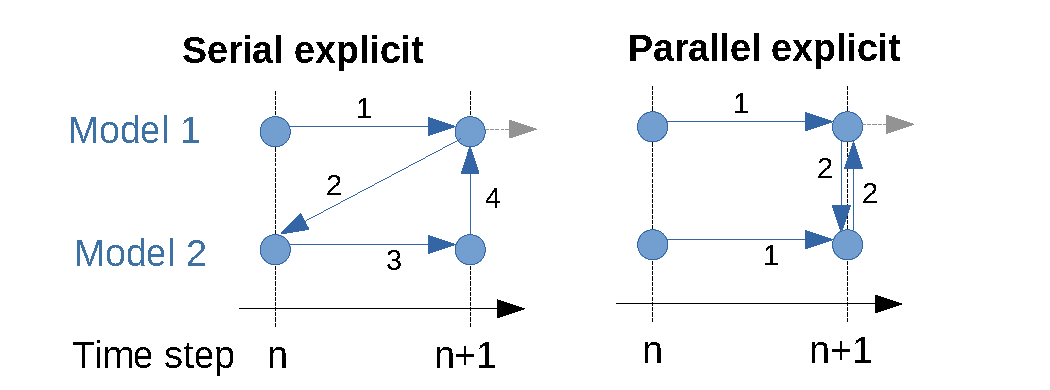
\includegraphics[width=10cm]{../figures/state-of-the-art/coupling/sequential approaches.pdf} 
\caption{Simple explicit update schemes used for multi-physics and multi-agent systems. In the serial update scheme (left), one of the models is evaluated first (1). The future state is passed to the other model (2) which uses the state for its prediction (3). The prediction is then passed back (4). In the parallel update scheme (right), the models are executed simultaneously. }
\label{fig:couplescheme}
\end{figure}


\subsubsection{Simulator coupling}
If models are located in different simulators, communication between the two simulators must be realized in addition to model coupling. 
Following approaches to exchanging data between two coupled simulators exist~\cite{gatzhammer-2014-cs}:

\begin{itemize}
\item File communication: simulators exchange data over files written to the harddisk. 
\item Socket communication: send and receive data over a network using communication protocols such as Transmission Control Protocol (TCP).
\item Message Passing Interface: intended for the communication of parallelized software in distributed systems.
\end{itemize}

The advantage of the file communication approach is that it does not require external communication libraries. The disadvantage is that the speed of the data exchange depends on the harddisk properties. If a large amount of data needs to be shared, it can take an infeasible amount of time. Therefore, file communication is often used as a fall-back solution when other communication methods fail~\cite[p.153]{gatzhammer-2014-cs}. 

Socket communication means exchanging data in a network. To manage a socket connection so-called co-simulation frameworks can be used. They manage the connecting process of the sockets and the data exchange. If a middleware is used, the simulator coupling is called `generic'~\cite{steinbrink-2017-cs}. Otherwise, the coupling is `specific', see Fig.~\ref{fig:cosimulationcoupling}. 


\begin{figure}[hbt!]
\centering
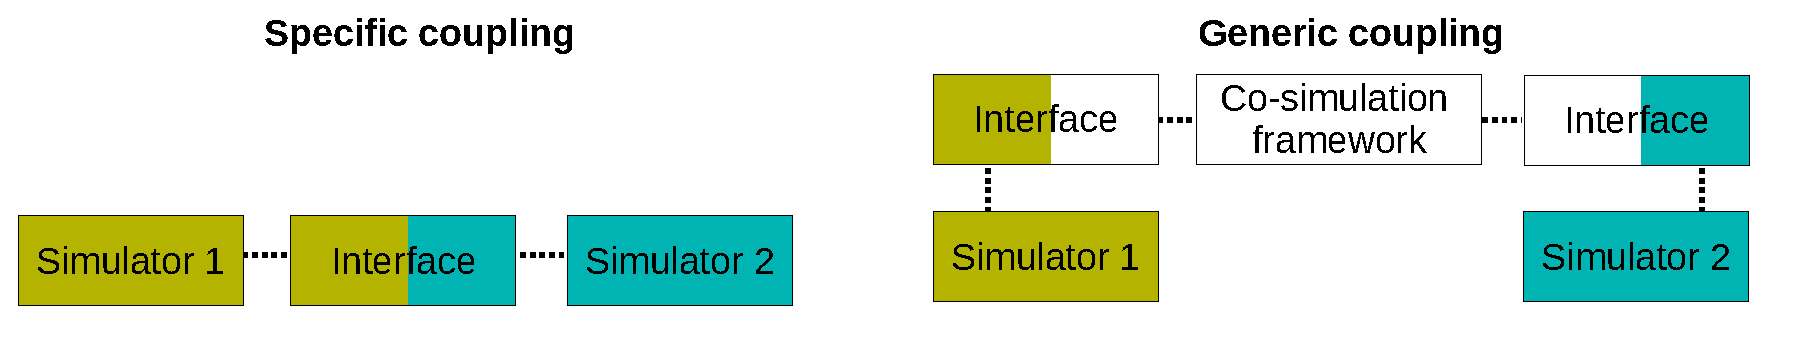
\includegraphics[width=\textwidth]{../figures/state-of-the-art/coupling/genericspecic.pdf} 
\caption[Overview on co-simulation.]{Generic and specific coupling. With a specific simulator coupling, the sockets of the simulators communicate directly over sockets in a network (left). In a generic coupling, a middleware manages the inter-process communication between simulators over sockets (right). For both types of coupling, suitable interfaces must be implemented. Own graphics inspired by~\cite{steinbrink-2017-cs}.}
\label{fig:cosimulationcoupling}
\end{figure}


\subsubsection{Validation of composite models}

Finally, I would like to briefly address the validation of composed models, assuming that the reader is familiar with the concepts of verification, validation, and calibration.  
The so-called composability theory deals with the question \enquote{[...] whether validity actually is preserved by composition. In other words, if two models are separately valid, can it be assumed that their composition is necessarily valid?}~\cite[p.63]{zhang-2019-cs}.
In his dissertation, Weisel~\cite{weisel-2004-cs} shows that a model, that is composed of two valid models, is not necessarily valid too. Only in some special cases, such as linear combinations, the composite model is valid under certain metrics~\cite{weisel-2004-cs}. 


Therefore, a composite model needs to be validated even when the component models have been validated. For this, conventional validation techniques can be used~\cite[p.76]{zhang-2019-cs}. Nevertheless, validating a model requires that empirical data is available. 



\subsection{Co-simulation frameworks and interfaces}
So far, one single crowd guidance system has been built using model and simulator coupling: CELLEVAC~\cite{lopez-2021-cdyn} for which the simulator AnyLogic was directly coupled with the commercial simulator Matlab. 

Apart from that, several middleware frameworks have been developed, see Fig.~\ref{fig:overviewcosimulation}. A middleware framework requires  to implement interfaces, see again Fig.~\ref{fig:cosimulationcoupling}. Therefore, it does not have an advantage over directly connecting simulators in terms of software engineering effort. Coupling simulators directly keeps the number of software dependencies low. For this reason, many direct couplings can be found in practice, see Tab.~\ref{tab:networkmiddleware}.


\begin{figure}[H]
\hspace*{-2cm}
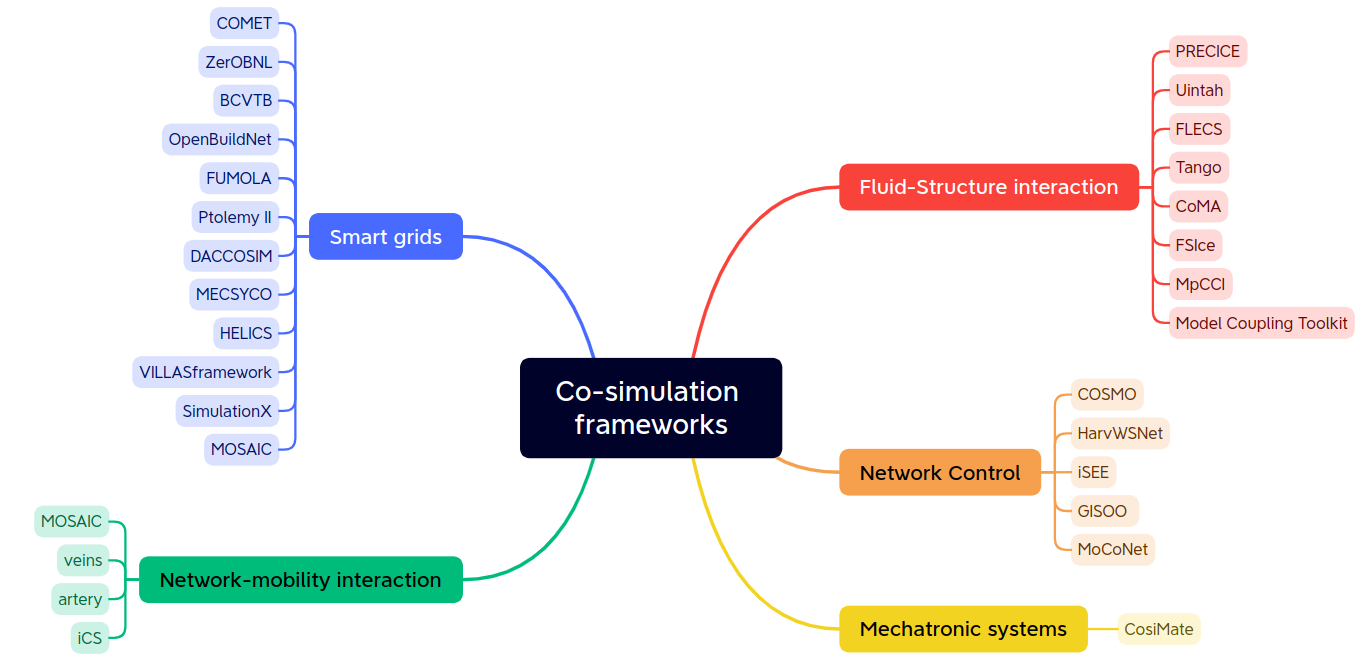
\includegraphics[width=1.2\textwidth]{./state-of-the-art/coupling/co-simulation-frameworks.png} 
\hspace*{2cm}
\caption[Overview on co-simulation frameworks]{Examples of co-simulation frameworks (middlewares). Co-simulation frameworks couple models from different simulation frameworks.
}
\label{fig:overviewcosimulation}
\end{figure}







\begin{table}[hbt!]
\centering
\begin{tabular}{lll}
 \hline 
 Framework & Mobility simulator & Network Simulator  \\ 
 \hline 
 Veins & SUMO & OMNeT++   \\ 
 Artery & SUMO & OMNeT++  \\ 
 iCS & SUMO & ns3  \\ 
 MOSAIC & SUMO, PTV Vissim & ns3, JiST/SWANS or OMNeT++  \\ 
 \hline 
 \end{tabular}  
 \caption[Simulator couplings]{Simulator couplings. The MOSAIC framework employs a generic coupling approach. Artery, iCS and Veins implement the Traffic Control Interface in the respective simulators (specific coupling). There is also one coupling with the commercial simulator PTV Vissim. }
\label{tab:networkmiddleware}
\end{table}

\newpage


For the specific coupling of mobile communication simulators and mobility simulators, the so-called Traffic Control Interface (TraCI) was introduced~\cite{wegener-2008-com}. The Traffic Control Interface couples a mobility simulator with a mobile communication simulator. The simulators exchange data over the Transmission Control Protocol (TCP). The TraCI protocol defines the structure of a message that is composed of a header and the content, see Fig~\ref{fig:tracimessage}. The content is either a request for data (How many vehicles are in the simulation?) or a command (Change the velocity of vehicle with $id=4$ to $20\,\text{km/h}$!). 


So far, only couplings  with the mobility simulator SUMO have been realized, see Tab.~\ref{tab:networkmiddleware}. The mobility models of the SUMO simulator are intended for large-scale scenarios: They cannot provide detailed trajectory data at a local scale. However, detailed data is necessary to evaluate the performance of a crowd guidance system. Therefore, the simulation frameworks listed in Tab.~\ref{tab:networkmiddleware} are not suitable for my investigations. I conclude that a novel simulation framework needs to be created that fits my needs.


\begin{figure}[hbt!]
\centering
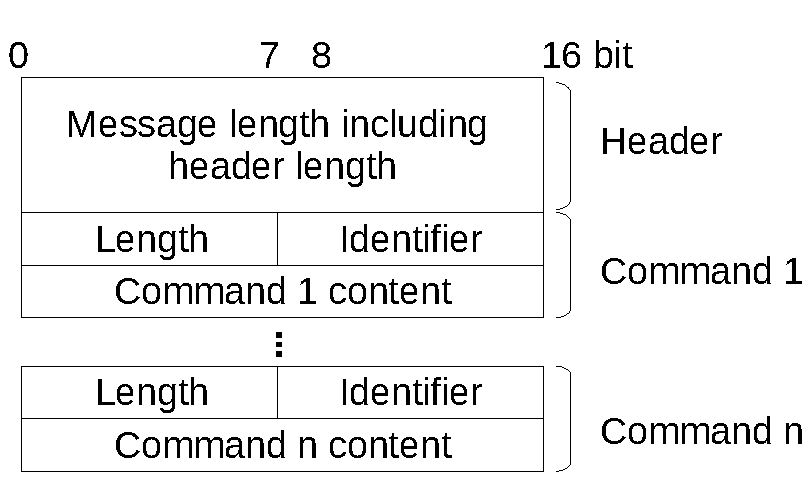
\includegraphics[width=7cm]{../figures/state-of-the-art/coupling/traci.pdf} 
\caption{Traffic Control Interface (TraCI) message. The message is communicated between the sockets of the mobile communication simulation and the socket of the mobility simulator  using the transfer communication protocol (TCP). TraCI messages are composed of a header and several commands. Own graphics inspired by~\cite{wegener-2008-com}.}
\label{fig:tracimessage}
\end{figure}






\section{Uncertainty quantification}
\label{sec:uq}
When evaluating simulation results, it is crucial to consider errors and uncertainties. Therefore, I look at uncertainty quantification methods in this section.
Several procedures exist to quantify uncertainties for which a wide theoretical foundation is available, see~\cite{smith-2014-math,xiu-2010-math}. 
One method is the Monte Carlo method~\cite{smith-2014-math}. The distribution of the uncertain parameter is approximated through a discrete sampling. The sample values are propagated through the simulation model which results in an output distribution, see Fig.~\ref{fig:uqforwardprop}. 
The Monte Carlo method requires many samples to approximate the distributions accurately, which is why applying it becomes infeasible when simulation runs take long~\cite{smith-2014-math}. This is the case for mobile network simulations that usually take several hours.
Therefore, I look at alternative uncertainty quantification methods that require less model evaluations.

In this section I look at surrogate-based uncertainty quantification with polynomial chaos expansions. I focus on two uncertainty quantification methods:
 \begin{itemize}
 \item Forward propagation: How uncertain is the model output due to uncertain parameters? 
 \item Sensitivity analysis: How influential are the uncertain parameters on the model output?
 \end{itemize}
 
The section is structured as follows: First, theory on polynomial chaos expansions is presented. In particular, it is explained how the coefficients of a polynomial chaos expansions can be determined. Then it is shown how uncertainty measures can be derived analytically from these coefficients.



\begin{figure}[hbt!]
\centering
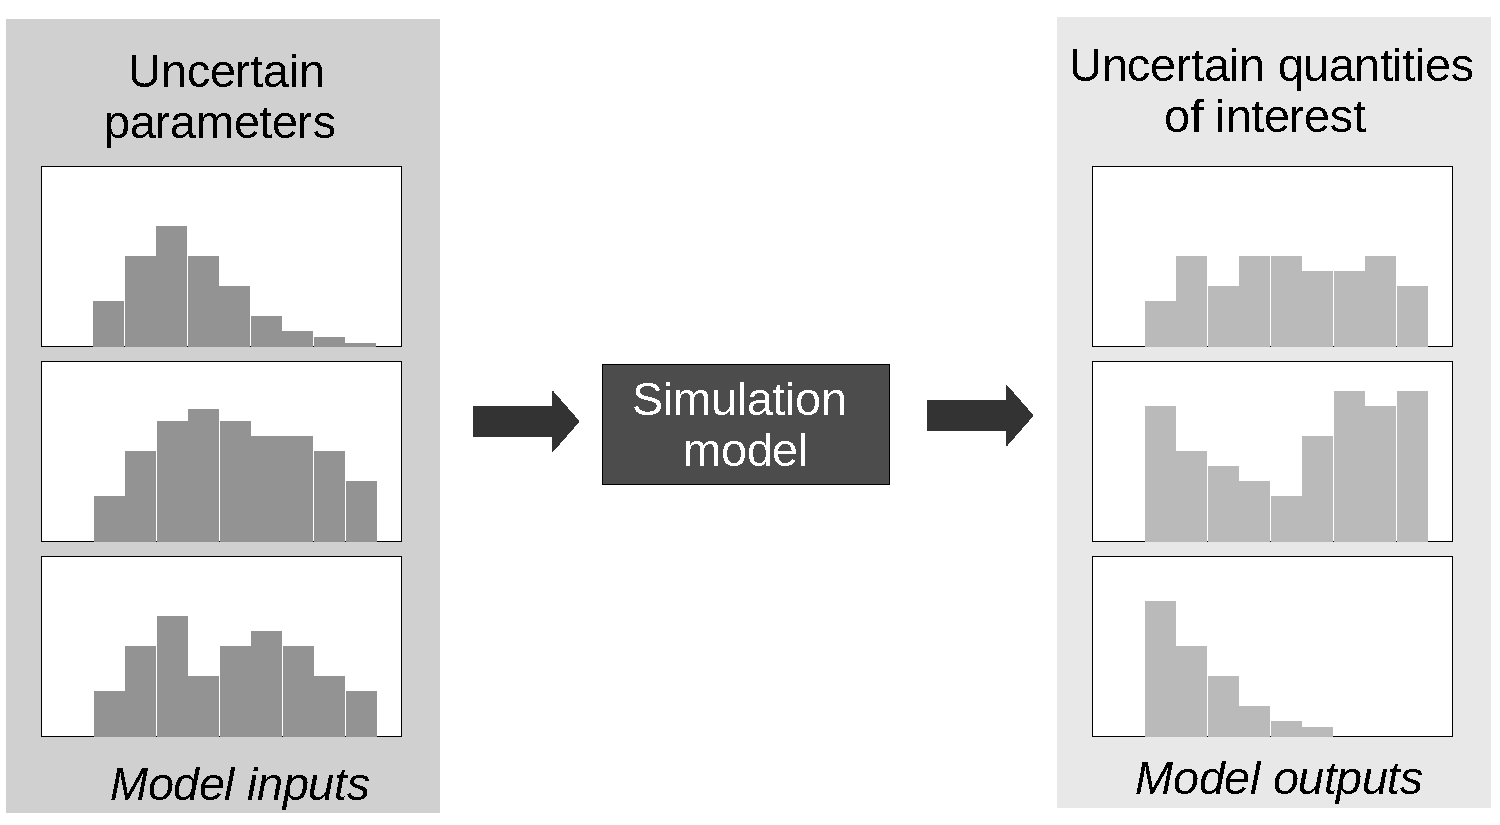
\includegraphics[width=10cm]{../figures/state-of-the-art/uq/overview.pdf} 
\caption{One method for uncertainty quantification is the Monte Carlo Method~\cite{smith-2014-math}. It can be used for forward propagation that aims to quantify the uncertainty of an output distribution. The uncertain input distributions (left) are propagated through a simulation model. Therefore, one gets an output distribution for which statistical moments can be computed. }
\label{fig:uqforwardprop}
\end{figure}



\subsection{Polynomial chaos expansion}

Polynomial chaos expansions, also known in literature~\cite{smith-2014-math} as spectral expansion, approximate an unknown model function $f$ that depends on the variable $t$ and the random variable $Z \in R^d$. Spatial, temporal, spatio-temporal, or any other deterministic dependencies are contained in $t$. The random variable $Z$ corresponds to an uncertain parameter of the simulation model $f$. A polynomial chaos expansion $f_N(t,Z)$ approximates $f(t,Z)$ using polynomial basis functions~\cite[p.67]{xiu-2010-math}:
\begin{equation}
f(t,Z) \approx f_N(t,Z) = \sum_{i \leq N}  \hat{f}_i(t) \phi_{i}(Z) \in P_N^d
\label{eg:polynmialchaosex}
\end{equation}
where $P_N^d$ is the space of polynomials of $Z$ of degree up to $N \geq 0$, $\hat{f}_i(t)$ are deterministic coefficients and $\phi_i$ are $M$ orthogonal polynomials that form a basis for the random component of the solution~\cite[p.209]{smith-2014-math}.

For any $t \in T$, the mean of $f$, denoted as $\mu_f(t)$, can be approximated by~\cite[p.67]{xiu-2010-math}:
\begin{equation}
\mu_f(t) \approx E[f_N(t,Z)] = \int \left(  \sum_{i \leq N}  \hat{f}_i(t) \phi_{i}(z)    \right) d F_Z(z) = \hat{f}_0(t)
\label{eq:meanpoly}
\end{equation}
where $F_Z(z)$ is the distribution of the random variable $Z$: $F_Z(z)=P(Z\leq z)$, see~\cite[p.64]{xiu-2010-math}.
Note that $\hat{f}_0(t)$ is the coefficient of the zero-order polynomial and has a similar function to the intercept in linear regression.

For any $t \in T$, the variance of $f$ can be approximated by~\cite[p.67]{xiu-2010-math}:
\begin{equation}
var(f(t,Z)) \approx \sum_{0  < i \leq N}  \hat{f}_i^2(t)    E[\phi_i^2(Z)]  = D_{PC}
\label{eq:varpoly}
\end{equation}

To determine the coefficients $\hat{f}(t)$, the Galerkin method, the collocation method, or the spectral method (projection) can be used. The Galerkin method is intrusive, which means that the simulation model needs to be adjusted, while the others are non-intrusive~\cite{smith-2014-math}. The spectral method requires fewer model equations than the regression-based collocation method as it only evaluates the model at particularly useful sample points. The errors of the mean and the variance convergence exponentially to zero over the number of expansion terms~\cite{xiu-2002-math}.

Each distribution type is assigned a specific polynomial type. This assignment is also known as the Wiener-Askey scheme, which extends the polynomial chaos expansions of Gaussian distributions to arbitrary distributions~\cite{xiu-2002-math}, see Tab. \ref{tab:polynomials}. The sample values are taken from quadrature tables and transformed to the respective parameter range. Therefore, the number of model evaluations equals the number of quadrature points.



\begin{table}[hbt!]
\centering
\begin{footnotesize}

\begin{tabular}{llll}
\hline 
 & Uncertain parameter $Z$ & Type of polynomial & Support \\ 
\hline 
Continous & Gaussian & Hermite & $]-\infty, \infty[$ \\ 
 & Gamma & Laguerre & $[0,\infty[$ \\ 
 & Beta & Jacobi & $[a,b]$ \\ 
 & Uniform & Legendre & $[a,b]$ \\ 
Discrete & Poisson & Charlier & $\{0,1,2,...\}$ \\ 
 & Binomial & Kryawtchouk & $\{0,1,2,...,N\}$ \\ 
 & Neg. binomial & Meixner & $\{0,1,2,...\}$ \\ 
 & Hypergeometric & Hahn & $\{0,1,2,...,N\}$ \\ 
\hline 
\end{tabular} 
\end{footnotesize}
\caption{  Distribution type of the uncertain parameter and referring type of polynomial~\cite[p.59]{xiu-2010-math}.  }
\label{tab:polynomials}
\end{table}

Standard polynomial expansions require that the model function $f$ and its derivatives are smooth~\cite{xiu-2009-math,feinberg-2018-cs}. Otherwise, the system behavior is not captured accurately due to Gibbs phenomena, that is, overshoots occur at transition points~\cite{feinberg-2018-cs}. To overcome this issue, variable transformation has been proposed: \enquote{The goal of the variable transformation is to create a new mapping which enables the response to be well approximated by a low-order polynomial chaos expansion.}~\cite{feinberg-2018-cs}. However, it is unclear how this can be implemented in practice if no information about $f$ or its differentiability is available. 


\subsection{Forward propagation and global sensitivity analysis}



Forward propagation aims to quantify the uncertainty of a quantity of interest due to uncertain parameters~\cite{smith-2014-math}. The uncertainty of the quantity of interest is quantified using the statistical moments~\cite[p.187]{smith-2014-math}. For a given polynomial chaos expansion, forward propagation cuts down to evaluating Eqs.~\eqref{eq:meanpoly}-\eqref{eq:varpoly} that describe how mean and variance depend on the coefficients of a polynomial expansion, see Fig~\ref{fig:uqexpansionstate}. 

\begin{figure}[hbt!]
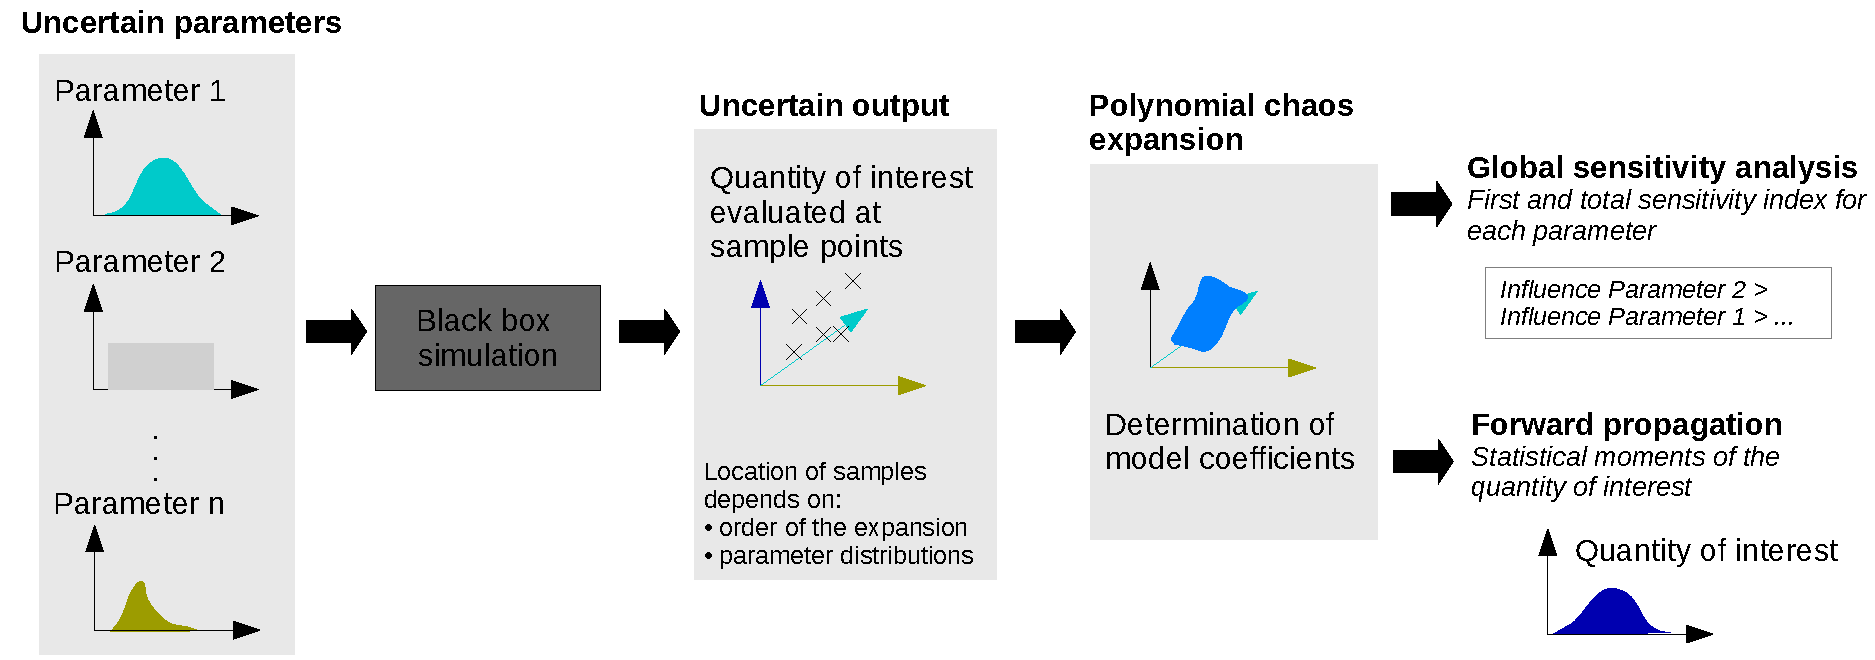
\includegraphics[width=\textwidth]{../figures/state-of-the-art/uq/polynomialchaosANDuq.pdf} 
\caption{Uncertainty quantification based on polynomial chaos expansions. Uncertain simulation parameters (left) are propagated through a black-box simulation model. The model evaluations are used to construct the polynomial expansion. With the coefficients, forward propagation and sensitivity analysis can be performed analytically. }
\label{fig:uqexpansionstate}
\end{figure}



Sensitivity analysis aims to quantify the influence of each parameter on a quantity of interest~\cite{smith-2014-math}. Global sensitivity analysis evaluates the parameter influence over the entire parameter range rather than the effect of local perturbations. One technique is the variance-based approach that can be applied to linear and non-linear functions~$f$~\cite{smith-2014-math}. The influence of each parameter on a quantity of interest~$f$ is quantified by so-called Sobol or sensitivity indices. Sudret et al.~\cite{sudret-2008-math} showed that sensitivity indices can be determined analytically from a given polynomial chaos expansion.


The first-order sensitivity index $S_i$ is defined as the ratio of the variance $D_i$ that is caused by the parameter $i$ only and the total variance $D$ of the quantity of interest:
\begin{equation}
S_i= D_i/D
\label{eq:si}
\end{equation}
The total-effect index $S_{T_i}$ is defined as ratio
\begin{equation}
S_{T_i}= D_{T_i}/D
\label{eq:siT}
\end{equation}
where $D_{T_i}$ is the variance caused by the parameter $i$ and its interactions~\cite{saltelli-2010-math} with the other parameters. The sensitivity indices can be derived analytically from its coefficients for a given polynomial chaos expansion. For this purpose, it is necessary to introduce the multivariate polynomial chaos expansion $f_N(t,\textbf{Z})$~\cite{mara-2021-math}:
\begin{equation}
f_N(t,\textbf{Z})  = \sum_{ \alpha \subset N^d}  \hat{f}_{\alpha}(t) \phi_{\alpha}(\textbf{Z})
\label{eq:multivariate}
\end{equation}
Note that the above equation is similar to Eq. \eqref{eg:polynmialchaosex} with the exception that the random variable $Z$ has been replaced by a set of random variables $\textbf{Z}$ and the index $i$ has been replaced the d-dimensional index $\alpha=\alpha_1 \alpha_2  ... \alpha_d \in N^d $ where $d$ is the number of parameters. The first sensitivity index $S_i$ can be represented as a function of the coefficients of the polynomial chaos expansions~\cite{mara-2021-math}:
\begin{equation}
S_i \approx \frac{  \sum_{ \alpha_i  > 0 }  \hat{f}^2_{ (0 ... \alpha_j ... 0) } } { \sum_{ \alpha_i  \subset  N^d}  \hat{f}^2_{\alpha} - \hat{f}^2_{(0...0)}  }
\end{equation}
Similarly, the total order indices can be represented as~\cite{mara-2021-math}:
\begin{equation}
S_{T_i} \approx \frac{   \sum_{\alpha_i  \subset  N^d: \alpha_i  > 0 }  \hat{f}^2_{  \alpha } } {  \sum_{ \alpha_i  \subset  N^d}  \hat{f}^2_{\alpha} - \hat{f}^2_{(0...0)}  }
\end{equation}
The index value evaluates the influence of a parameter. An index value of 1 means a high influence, and a value of 0 means a low influence.
Standard libraries, such as the Python package Chaospy, provide implementations for the construction of the polynomial chaos expansion and the computation of the sensitivity indices.



\section{Summary}


In this chapter I presented and analyzed state-of-the-art approaches for crowd management. A definition for crowd management was provided, differentiating it from crowd control. Then metrics for evaluating pedestrian traffic were discussed. To redirect crowds efficiently, I looked at psychological theories about crowd behavior. I found that social identities affect crowd behavior and, therefore, should be considered when providing guidance information. 


My review of crowd-sensing procedures showed that a variety of methods exist, including methods that utilize mobile communication. However, none of the approaches can measure flows or the spatial distribution of pedestrians using direct communication technology. I concluded that new methods are needed. 


The review of algorithms that compute signals to guide crowds based on current environmental information showed that the proposed algorithms were either customized to scenarios and, therefore, not transferable or were tested under the assumption that people always follow instructions, which is wrong. I concluded that algorithms are needed that can be applied to arbitrary scenarios. They should be tested under realistic conditions, that is, not all people follow instructions.


In the second part I looked at modeling and simulation approaches. My review of crowd models showed that several validated models exist for modeling the movement behavior. However, no generally applicable route choice model is available for modeling route choice behavior. Therefore, I concluded that a new modeling approach is needed to model route choice in a crowd guidance system.
In addition I found that although there are several approaches to modeling psychological behavior and communication, none of them have been used to redirect crowds in a crowd guidance system. Therefore, transferring these methods is necessary. 


Then I looked at the modeling and simulation of direct communication in mobile networks according to four mobile standards that specify direct communication: The two IEEE standards 802.11p and 802.11bd that enable direct communication in WLAN ad hoc networks, and the LTE and 5G standards of the 3rd Generation Partnership Project intended for cellular communication with or without base station that allocates resources. I looked at different modeling approaches for the radio channel and gave an overview of standardized channel models released by the mobile communication community. These models can be employed for my investigations, and no further development is necessary. 


Since a crowd management system is made up of various components, I next looked at approaches for coupling models and simulators. I presented two types of model couplings and discussed time-stepping and update procedures. I found that, due to the fact that a crowd guidance system based on direct communication technology is novel, a suitable update scheme needs to be found. Then I looked at the inter-processes communication, that is, how simulators exchange data. I found that there are middleware simulation frameworks and standardized interfaces available, but there is no simulation framework available that allows one to simulate a crowd guidance system using direct communication technology. Therefore, I concluded that a simulation framework needs to be created that I can use for my investigations. 

Finally, I presented a procedure for quantifying uncertainties in simulation results due to uncertain simulation parameters that I use in my investigations.

